\section{Introduction}
\label{sec:introduction2}

The concept of sustainable forest management (SFM) has long been a central theme of Crown (public) forest policy in Canada \citep{ccfm2008vision}. In concrete terms, sustainable forest management policy is implemented via silviculture treatments, notably harvesting treatments. According the the \emph{Criteria and Indicators of Sustainable Forest Management in Canada} \citep{ccfm2006criteria}, harvesting is generally deemed to be sustainable if it is below annual allowable cut (AAC) level. 

% In the case of forest management on public land, the relationship between government steward and industrial fibre consumer can be described as an instance of the \emph{principal-agent problem}.
% Government stewards (the principal) manage the land and grant timber harvesting licenses to industrial fibre consumers (the agent). The principal develops long-term forest management plans. Achievement of the principal's long-term goals depends requires that his plan be executed exactly. These plans are essentially composed of a sequence of harvesting treatment prescriptions, assuming a certain type, location, and timing for each treatments. The agent is typically responsible for planning and executing the short-term harvesting activities, which allow him to procure fibre for his mills. For a number of reasons, including logistical and economical factors, the agent will not willingly adhere exactly to the harvesting treatment sequence in the long-term plan. The antagonism in this principal-agent problem stems from the principal's dependency to implement the harvesting activities that constitute his long-term plan.

AAC is commonly determined using mathematical optimization models. 
The classic Model I \citep{davis2001forest-ch13} wood supply model formulation is the \emph{de-facto} standard wood supply planning tool in many jurisdictions.  
This classic model formulation finds the maximum indefinitely-sustainable\footnote{These models actually have a finite planning horizon. Typical rule-of-thumb horizon length choice would double the average timber rotation period. For example, a typical rotation period in the boreal forest is 75 years; a common wood supply model planning horizon is 150 years, discretized into 30 five-year periods. Planners assume that simulating sustainability over this horizon is sufficient to demonstrate indefinite sustainability.} harvest level, based on the implicit assumption that local fibre demand will always exceed supply.
In other words, the classic model assumes that all available fibre will be consumed in every planning period, regardless of quantity, quality, cost, or value creation potential.
In practice, this infinite-demand assumption is rarely respected.
Consequently, the classic wood supply optimization model tends to systematically over-estimate fibre consumption. Thus, we can expect that the principal's plan will never be executed, and that the long-term state of the forest may be quite different from that predicted by the classic wood supply model.

In this context, \citet{paradis2013risk} show that the classic model may fail when AAC exceeds industrial demand, and recommend further constraining the wood supply model based on anticipated fibre demand. This paper presents a novel bilevel extension of the classic formulation, which explicitly anticipates industrial fibre consumption using a subordinate optimization model to capture the agent's profit-maximization behaviour.
%We implement this recommendation using a bilevel model formulation.
Our bilevel model finds the maximal species-wise even-flow wood supply levels that we anticipate will be entirely consumed by a profit-maximizing industrial fibre consumer, thereby reducing the magnitude of the negative fibre consumption bias (relative to the classic wood supply model formulation).  
We show that the solution space induced by the bilevel reformulation is non-convex, which makes the general case difficult to solve exactly. 
We proceed to describe a special convex case of the problem that can be solved to global optimality using a decomposition-based solution methodology. 
%Finally, we test our solution methodology on a dataset of realistic size and complexity, to demonstrate algorithmic convergence and problem tractability.

The objectives of this study are to (a) compare the long-term performance of the classic and bilevel wood supply optimization model formulations after several rolling-horizon planning cycles, and (b) provide recommendations for improving the credibility of the wood supply planning process.

\section{Background}
\label{sec:background2}

The term \emph{wood supply planning} describes the process by which AAC is determined. In practice this typically amounts to solving a linear programming (LP) optimization model, which maximizes AAC subject to even-flow constraints \citep{gunn2007models}. Provincial government authorities allocate timber licences (TL) to industrial fibre consumers. These TLs set (species-wise) upper bounds on periodic harvest volume, however there is typically no policy requirement to set matching lower bounds. 

%This implies that 

%Wood supply planning plays an important role in sustainable forest management. This is particularly true on Crown (public) forest land in Canada, where government steward manage the forest resource on behalf of the Canadian people. 

Timber licences are typically valid for a pre-determined period (e.g., 5 years), after which point licenses may be renewed, subject to re-evaluation of species-wise AAC. Figures \ref{fig:aac} and \ref{fig:jointdist}(a) show species-wise Canadian AAC data from 1990 to 2012. Although there is some fluctuation over time, total national AAC has been relatively stable during this period.

For a variety of economic and logistic reasons, some portions of AAC are not attractive to timber licensees and are not harvested. Figures \ref{fig:aac_consumption} and \ref{fig:jointdist}(b) show species-wise proportion of Canadian AAC consumption from 1990 to 2012. On average, 80\% of softwood AAC is consumed, versus 45\% of hardwood AAC, indicating a clear industrial preference for softwood. Consumption rates for both species groups show similar variability. Softwood AAC consumption appears to be following a slight downward trend, whereas hardwood AAC consumption appears to be on the rise. 

\begin{figure}[h]
  \centering
  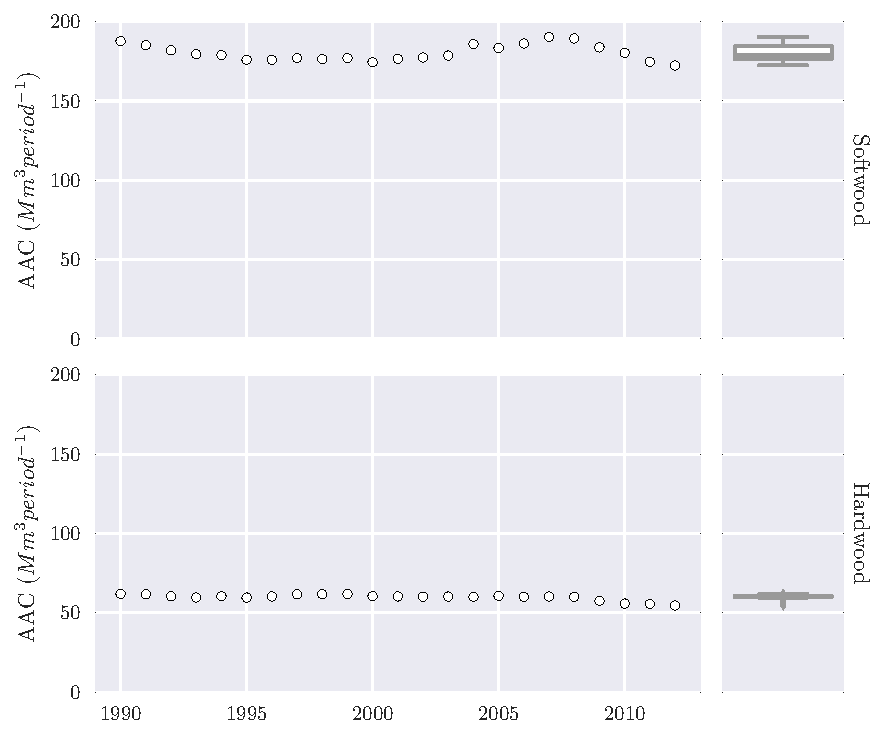
\includegraphics[width=\textwidth]{images/aac}
  \caption{Species-wise AAC consumption for period 1990 to 2012}
  \label{fig:aac}
\end{figure}

\begin{figure}[h]
  \centering
  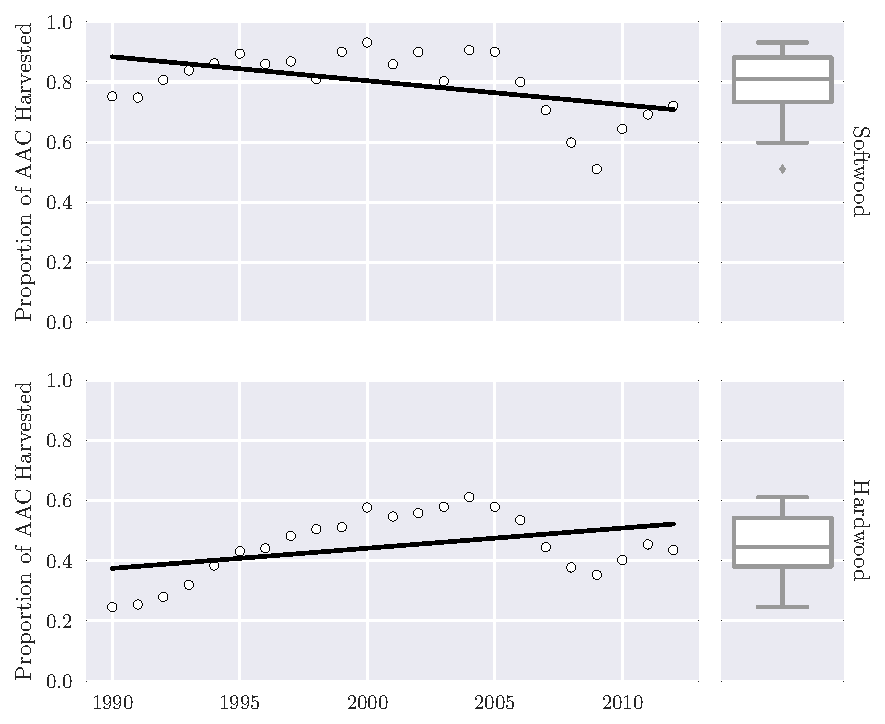
\includegraphics[width=\textwidth]{images/aac_consumption}
  \caption{Proportion of species-wise AAC consumed for period 1990 to 2012}
  \label{fig:aac_consumption}
\end{figure}

\begin{figure}[t]
    \centering
    \subfloat[AAC]{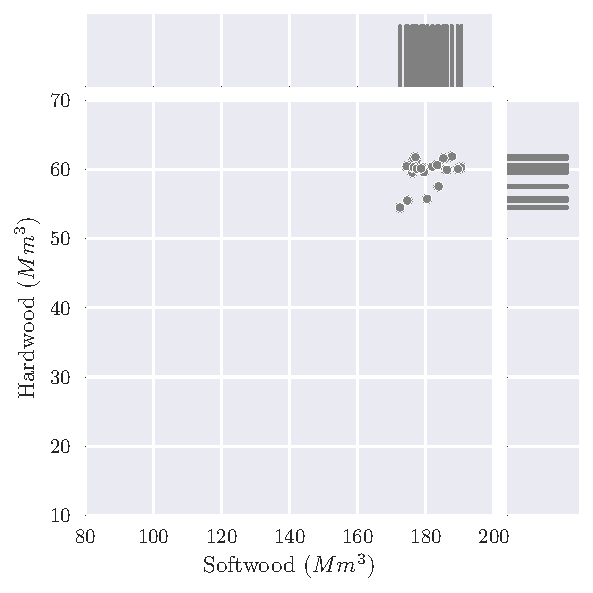
\includegraphics[width=0.5\textwidth]{images/aac_jointplot}}
    \subfloat[Fibre consumption]{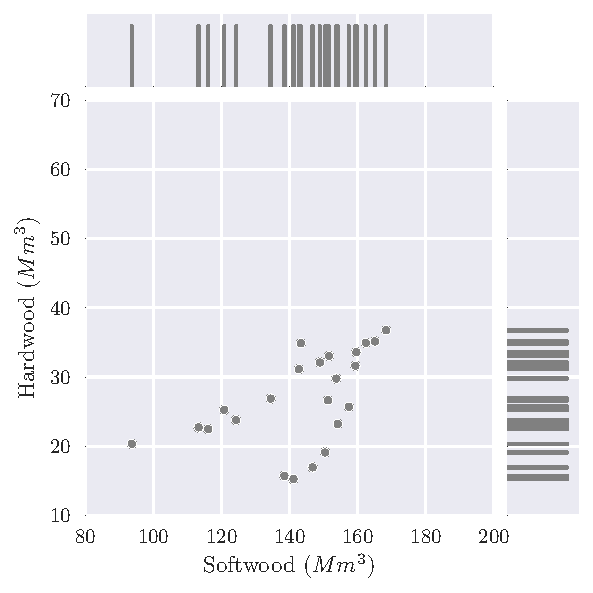
\includegraphics[width=0.5\textwidth]{images/harvest_jointplot}}
  \caption{Species-wise joint distributions of AAC and harvest volume for period 1990 to 2012}
  \label{fig:jointdist}
\end{figure}

% \begin{figure}[t]
%     \centering
%     \begin{subfigure}[t]{0.5\textwidth}
%         \centering
%         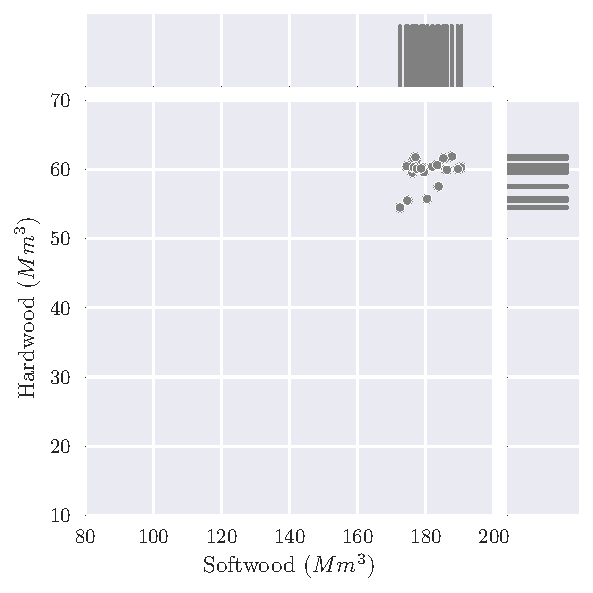
\includegraphics[height=\textwidth]{images/aac_jointplot}
%         \caption{AAC}
%     \end{subfigure}%
%     \begin{subfigure}[t]{0.5\textwidth}
%         \centering
%         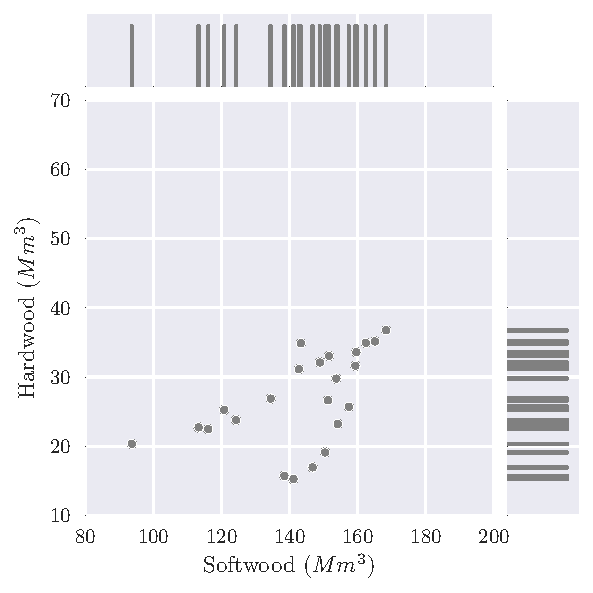
\includegraphics[height=\textwidth]{images/harvest_jointplot}
%         \caption{Harvest Volume}
%     \end{subfigure}
%   \caption{Species-wise joint distributions of AAC and harvest volume for period 1990 to 2012}
%   \label{fig:jointdist}
% \end{figure}


The data show a species-skewed negative consumption bias, relative to AAC, which is related to the infinite-demand assumption implicitly embedded in the classic wood supply optimization model formulation. 
%which is the \emph{de facto} standard tool used by government authorities to determine AAC on Crown land. 
\citet{paradis2013risk} estimate the impact of this bias, using a sequence of 30 two-phase rolling-horizon planning cycles\footnote{The first phase simulates determination of AAC by government officials, and the second phase simulates consumption of a profit-maximizing subset of available fibre by forest products industry firms.}, and show that consuming a species-skewed subset of AAC can induce future wood supply failures under certain conditions. They conclude that the wood supply planning process currently in place on Crown land in Canada does not provide credible assurance of long-term sustainability of the wood supply. Given the pervasiveness of the species-skewed negative consumption bias, the classic wood supply optimization model formulation does not constitute a rational basis for the implementation sustainable forest management. 

%---



% \subsection{Wood Supply Planning}

% \subsection{Principal-agent Problem}

% \subsection{Bilevel Optimization}

For management and planning purposes, the forest landscape is subdivided into \emph{stands}. 
The \emph{stand} is the basic silviculture decision unit, and can be described as a contiguous forested area with uniform vegetation and growth characteristics. 
Projection of future forest condition and fibre availability is based on aggregated result of stand-level growth and yield simulation. 
This requires four distinct types of information: (a) hypothetical detailed inventory of current forest condition (i.e., stand ages and types), (b) hypothetical projection of stand condition over time for each type\footnote{Foresters typically refer to these as \emph{yield curves}.}, (c) hypothetical state transitions induced by stand events (i.e., shift in stand age and stand type), and (d) hypothetical intensity, location and timing of planned future stand events (e.g., clear-cut harvesting of stand $x$ in planning period $i$). 

%High cost of collecting and compiling inventory, yield curve, and transition inputs is matched with heightened awareness of sampling error. 
%Particular attention is paid to minimizing estimation bias \todo{Add references showing research on impact of wood supply model input error.}. 
%Thus, estimation error tends to cancel out for the first three data types \citep{ouhimmou2010robust}. 

Wood supply optimization models typically use the first three information types (i.e., starting inventory, yield curves, and state transitions) as input, leaving the fourth information type (location and timing of future stand events) as variables in the objective function. 
%The c is often obtained from the output of wood supply optimization models. implicitly embedded in the objective function and constraints of the classic wood supply planning model. 
%The implicit nature of the future harvest hypotheses on wood supply analysis has received relatively little attention in the literature. 
Assembling this information into a coherent model, and subsequent analysis of model output, is referred to as the \emph{wood supply planning problem}. 
We focus on a particular problem variant, which we call the \emph{distributed wood supply planning problem}, where the roles of forest land owner and industrial fibre consumer are played by independent agents. 
This is a common situation in Canada and other jurisdictions, where public forest land is managed by government stewards on behalf of the general population.

%\citet{paradis2013risk} present an illustrative case study showing that the common "maximal even-flow harvest volume" wood supply model formulation implicitly assumes that aggregate fibre industrial demand exceeds potential fibre supply throughout the planning horizon. This assumption does not hold in many instances. Using a two-phase iterative simulation, the authors show that systematic over-estimation of harvesting activity in this wood supply model formulation can have a negative impact on both credibility of long-term demonstration of sustainability and stability of industrial fiber supply.

%Based on these findings, we propose to extend the "maximal even-flow harvest volume" wood supply model formulation to include explicit anticipation of industrial fibre consumption behaviour. 

The classic wood supply planning model formulation 
%(see \citet{paradis2013risk} for a detailed description of formulation) 
does not explicitly consider industrial fibre-consumption behaviour. Instead, it implicitly assumes infinite demand (i.e., all harvested fiber will be consumed, regardless of quantity, quality, species, price, or other considerations). This assumption is not coherent with available data in some jurisdictions, where historical fibre consumption is systematically lower than maximum potential wood supply \citep{ccfm2005wood}.  This bias compromises credibility of the wood supply planning process.

We aim to improve the long-term wood supply planning model formulation by explicitly anticipating industrial fibre consumption behaviour. To do so, we can describe the distributed wood supply planning problem, from game-theoretic perspective, as an instance of the principal-agent problem. 
% Stackelberg game \citep{stackelberg2010market, olsder2009phenomena}. 
The role of \emph{principal} is played by the forest owner (or government steward), and the role of \emph{agent} is played by the industrial fibre consumer. 
%Although we embed our model in an iterative simulation framework, we disregard the repeated nature of principal-agent interaction (i.e, we assume a static or ``one shot'' game, with no dynamic evolution of player behaviour induced by game repetition).
%The principal wishes to offer the biggest perpetually-renewable wood supply contract possible. 
%When the principal uses the classic wood supply optimization model, he fails to account for the agent's willingness to consume all the fibre offered.

%%%%%%%%%%%%%%%%%%%%%%%%%%%%%%%%%%%%%%%%%%%%%%%%%%%%%%%%%%%%%
% TO DO: summarize PA in forestry literature...
%%%%%%%%%%%%%%%%%%%%%%%%%%%%%%%%%%%%%%%%%%%%%%%%%%%%%%%%%%%%%

\section{Source of Antagonism}

The principal has the long-term responsibility to ensure a sustained wood supply (hence the even-flow constraints in the wood supply model), but aims to maximize economic activity from exploitation of the forest resource (hence the wood-supply-maximization objective function).
The agent aims to maximize short-term profit from transformation of wood supply into forest products.
Antagonism between the principal and agent is linked to either (a) binding agent capacity constraints or (b) the presence of negatively-valued subsets of the wood supply. 
Either of these factors will prevent the profit-maximizing agent from consuming the entire wood supply, which in turn induces the problematic negative consumption bias described in \citet{paradis2013risk}.

The test dataset used in the computational experiments presented later in this paper features binding agent capacity constraints.
Our test dataset has two lines (which we will refer to as \emph{hardwood} and \emph{softwood}, based on an aggregation of tree species that grow in our test forest).
All the hardwood harvested from the forest must pass through a single hardwood sawmill.
The hardwood sawmill capacity is approximately one third of the maximum sustainable hardwood supply level determined by the principal using the classic wood supply optimization model.
The softwood line is profitable and has sufficient capacity to process the entire softwood supply offered by the principal.
The agent therefore has an incentive to utilize his entire softwood allocation, but limit his hardwood consumption to the capacity of the hardwood sawmill.
We have only permitted clear-cut harvesting in our test model, which means the agent only has take-all and leave-all options for each harvestable forest unit.
In order to achieve the correct hardwood/softwood mix in his harvesting plan, the agent may select harvest units that have a lower proportion of hardwood than the harvest units appearing in the first period of the principal's optimal wood supply solution.
This species-biased deviation from the principal's wood supply plan increases risk of future wood supply shortages.

In the case of wood supply offers with negatively-valued subsets, the only way the principal has to motivate the agent to act is by allowing him to harvest part of the forest (i.e., the agent can choose to consume any subset of wood supply offered by the principal). 
In practice, it is difficult (impossible) for the principal to force the agent to consume timber at a net loss, so this is a real problem. 
The principal is incited to propose plans where part of the output is not interesting for the agent, as this allows him to increase his wood supply offer (this is desirable, given his objective function). 
Including this negatively-valued part in the short-term wood supply allows the principal to increase the long-term wood supply offer\footnote{For example, simulating harvesting of relatively unproductive or over-mature parts of the forest and regenerating them into higher-productivity stands in a wood supply model may increase the availability of fibre in a future time period. This \emph{allowable cut effect} is a well documented forest policy instrument. For more information, see \citet{luckert1995allowable}.}.
However, the agent only plans his consumption on a short-term basis, and has no incentive to consume the negatively-valued subset of wood supply.
It may be impossible for the principal to offer the globally optimal plan \emph{and} force the agent to use all of the wood offered. 
By not consuming the uninteresting part of the supply, the agent may compromise the principal's long term plan.

We illustrate this second source of antagonism with an example. % (see Figure \ref{ref:stablestate}).
Suppose the principal $P$ can offer $H_1$ to the agent $A$, which has a value $v(H_1) = 10M\$$. 
To this offer, the principal can add $H_2$, which has a value $v(H_2) = 2M\$$.
However, $H_1$ and $H_2$ can only be consumed sustainably if they are bundled with $H_3$, which has a value $v(H_3) = -1M\$$. 
The best long-term solution for both parties is for the agent to consume $H_1$, $H_2$ and $H_3$ for $v(H_1 \cup H_2 \cup H_3) = 11M\$$.
However, the principal knows that if he offers all three lots, the profit-maximizing agent will only take $H_1$ and $H_2$ for $v(H_1 \cup H_2) = 12M$.
The principal knows that this is unsustainable, so he only offers $H_1$ which is sustainable but has a lower value of $10M\$$.

Note that if the principal could bundle the uninteresting part with a more interesting surplus, then the antagonism would disappear.
However, this bundling would require a more highly-constrained contract binding the agent to the principal.
This bundling option is not typically available to the principal in practice, leaving him with no rational choice but to lower the wood supply offer until the agent willingly consumes it all.
Determining the maximum species-wise even-flow wood supply offer that will be totally consumed by the agent is not a trivial problem.
The antagonism between the two levels can induce non-convexity in the solution space, when we constrain the principal's problem such that a wood supply contract is principal-feasible only if the agent consumes it entirely.

% \begin{figure}[h]
%   \centering
%   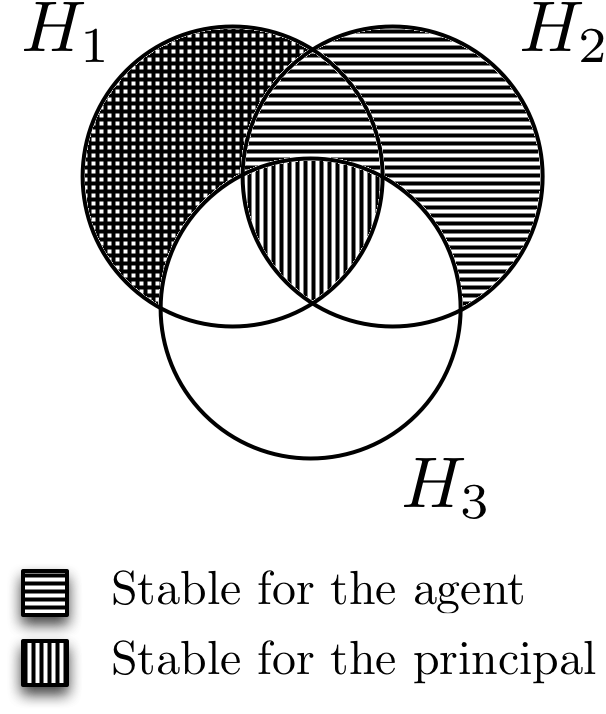
\includegraphics[width=50mm]{images/venn_stablestate}
%   \caption{Illustration of stable state for principal and agent}
%   \label{fig:stablestate}
% \end{figure}

\section{Non-Convexity of Bilevel Solution Space} 

\todo{Should we consider moving the detailed proof to an appendix?}

Before we present a formal mathematical formulation of the bilevel optimization problem, we provide a simple counter-example illustrating potential convexity problems (see Figure \ref{fig:counterexample}). The context for our counter-example is a simple setup where the principal offers a supply of hardwood and softwood to the agent. 
The agent must willingly consume the entire wood supply offer for a given solution to be principal-feasible.

The agent is actually composed of two independent sub-agents (softwood and hardwood lines). 
This is similar to the test dataset used in the computational experiments we present later in this paper.
Each sub-agent maximizes his own profit (i.e., is not willing to reduce his profit for the benefit of the other).
There are three types of transformation processes: boards, paper, and cogeneration.
The \emph{boards} process is equally profitable for both lines ($+50\,\si{\$\per\cubic\metre}$ for both softwood and hardwood), and has a transformation capacity of two input units for each line.
The \emph{paper} process is profitable for both lines, but at different rates ($+50\,\si{\$\per\cubic\metre}$ for the softwood line, $+10\,\si{\$\per\cubic\metre}$ for the hardwood line); it has a transformation capacity of three input units for each line.
The \emph{cogen} process is marginally profitable for for the softwood line ($+1\,\si{\$\per\cubic\metre}$), and marginally unprofitable for the hardwood line ($-1\,\si{\$\per\cubic\metre}$); it has a transformation capacity of one input unit for each line.

Transforming inputs using the paper process requires utilization of a common resource for both lines.
There is a difference in line-wise efficiency for utilization of the common resource.
The softwood line utilizes two units of the common resource for each unit of input transformed, whereas the hardwood line is twice as efficient.
Problems with non-convexity of the solution space may arise when this common resource becomes saturated.

The counter-example starts with a solution offer of $4$ units of softwood and $4$ units of hardwood.
The agent consumes the entire offer, for a profit of $\$320$. 
Consider a slight perturbation that alters the solution by $+2$ units softwood and $-2$ units of hardwood; this produces the globally optimal solution, for a profit of $\$351$. 
We will show that this $(+2S,-2H)$ bundled move, while still increasing the value for the agent, goes outside of the stable solution space.
Next, consider a smaller perturbation that alters the solution by $+1$ unit of softwood and $-1$ unit of hardwood.
In this case, the agent will not consume the entire offer (he will not consume the unprofitable unit of hardwood that would go to the cogen process).
This is an infeasible solution from the perspective of the principal, as the bilevel model formulation requires the principal to consider only wood supply offers that will be entirely consumed by the agent. Given that all three points (i.e., $(0S, 0H)$, $(+1S, -1H)$, $(+2S, -2H)$) located along a line in solution space, infeasibility of intermediate point $(+1S, -1H)$ proves non-convexity\footnote{By definition, given a line segment whose endpoints lie inside a convex space, it is not possible for any point along this line segment to lie outside the convex space. }\todo{Hopefully the footnote clarifies sufficiency of our counter-example as proof of non-convexity of the general problem case.}.

Even the simplest bilevel optimization problems are known to be $\mathcal{NP}$-hard, and non-convex solution spaces are common \citep{dempe2003annotated, colson2007overview}. 

%\todo{Has this condition been clearly defined yet earlier in the text?}

% The the prototype for this methodology was developed under the incorrect assumption that the solution space for combined problem P3 was convex.
% In fact, the solution space for problem P3 is non-convex, which is common in bilevel programs \citep{dempe2003annotated}.

\begin{figure}[H]
  \centering
  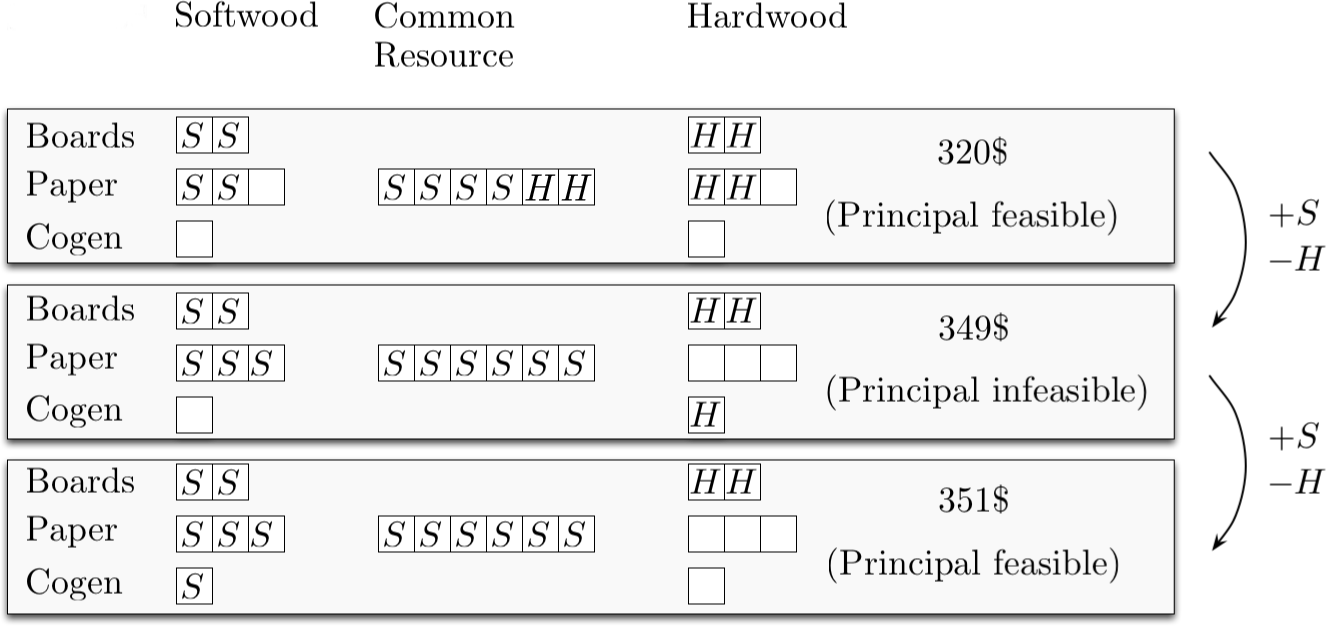
\includegraphics[width=\textwidth]{images/counterexample_edited2}
  \caption{Simple counter-example illustrating non-convexity of bilevel problem solution space}
  \label{fig:counterexample}
\end{figure}


% From olsder2009phenomena:
% In [13], one can for instance read: “It is a remarkable feature of these problems (i.e., contract design games) that the leader always takes all, pushing the follower to zero utility”.
% 13. Selanie, B.: The Economics of Contracts. MIT Press, Cambridge (2000)
%
% This seems to be the case for our model as well; the principal pushes the agent to the break-even point in an effort to maximize AAC.

%We show that tightening the gap between planned and implemented harvesting activities improves both credibility and performance of the distributed wood supply planning process.

\section{Mathematical Formulation}
\label{sec:formulation2}

This section describes the bilevel optimization problem formulation. We use the bilevel programming terminology found in \citet{colson2007overview}.

\subsection{General Case}

We present a mathematical formulation for the general case. First, we define some symbols which will be used to formulate the principal and agent models.

\begin{align*}
\intertext{Let}
\Theta &\colonequals  \text{set of extreme principal feasible solutions}\\
\Phi &\colonequals  \text{set of extreme agent feasible solutions}\\
O &\colonequals \text{the set of forest outputs}\\
R &\colonequals \text{set of resources}\\
\gamma_{\theta,o} &\colonequals \text{quantity of output $o \in O$ produced by the principal solution $\theta \in \Theta$}\\
\alpha_{\phi,r} &\colonequals \text{quantity of resource $r \in R$ consumed by the agent solution $\phi \in \Phi$}\\
\delta_{\phi,o} &\colonequals \text{quantity of output $o \in O$ consumed by the agent solution $\phi \in \Phi$}\\
v_{\theta} &\colonequals \text{value of solution $\theta \in \Theta$ for the principal}\\
w_{\phi} &\colonequals \text{value of solution $\phi \in \Phi$ for the principal}\\
g_{\phi} &\colonequals \text{value of solution $\phi \in \Phi$ for the agent}\\
u_r &\colonequals \text{maximal amount of resource $r \in R$}\\
\intertext{represent the parameters, and}
 x_{\theta} &\colonequals \text{proportion of the final principal solution built from principal solution $\theta \in \Theta$}\\
y_{\phi} &\colonequals \text{proportion of the final agent solution built from agent solution $\phi \in \Phi$}\\
\mu_o &\colonequals \text{dual price of output $o \in O$}\\
\pi_r &\colonequals \text{dual price of resource $r \in R$}\\
\intertext{represent the variables.}
\end{align*}

\begin{align} 
  \intertext{The primal formulation of the agent's optimization problem is}
    z_A(x) \colonequals \boldsymbol{\max} \sum_{\phi \in \Phi} g_{\phi} y_{\phi} \\
    \shortintertext{\textbf{subject to} \nonumber} \\
     \sum_{\phi \in \Phi} \alpha_{\phi,r} y_{\phi} & \leq u_r , & \forall r \in R \\
     \sum_{\phi \in \Phi} \delta_{\phi,o} y_{\phi} & \leq d_o = \sum_{\theta \in \Theta} \gamma_{\theta,o} x_{\theta} , & \forall o \in O \\
     \sum_{\theta \in \Theta} x_\theta & = 1 \\
     \sum_{\phi \in \Phi} y_\phi & = 1 \\
     y & \geq 0 \\
    \intertext{The dual formulation of the agent's optimization problem is}
   z_A(x) \colonequals \boldsymbol{\min} \sum_{r \in R} u_r \pi_r + \sum_{o \in O} d_o \mu_o \\
    \shortintertext{\textbf{subject to} \nonumber} \\
     \sum_{r \in R} \alpha_{\phi,r} \pi_r + \sum_{o \in O} \delta_{\phi,o} \mu_o & \geq  g_{\phi} , & \forall \phi \in \Phi \\
    \pi, \mu & \geq 0 
\end{align}

The global solution is stable for both the principal and the agent if the following condition is met, expressing equality of output production (by the principal) and output consumption (by the agent).

\begin{equation}
\sum_{\phi \in \Phi} \delta_{\phi,o} y_{\phi}  = \sum_{\theta \in \Theta} \gamma_{\theta,o} x_{\theta}
\end{equation}

A stable formulation can be obtained by combining the primal and dual agent problems, and requiring equality on the output consumption constraint.

\begin{align} 
    z_A(x) \colonequals \boldsymbol{\max}  \sum_{\phi \in \Phi} g_{\phi} y_{\phi} \\
    \shortintertext{\textbf{subject to} \nonumber} \\
    \sum_{\phi \in \Phi} \alpha_{\phi,r} y_{\phi}  - s_r  & = u_r, & \forall r \in R \\
    \sum_{\phi \in \Phi} \delta_{\phi,o} y_{\phi} & = \sum_{\theta \in \Theta} \gamma_{\theta,o} x_{\theta} , & \forall o \in O \\
    \sum_{r \in R} \alpha_{\phi,r} \pi_r + \sum_{o \in O} \delta_{\phi,o} \mu_o - \sigma_\phi  & = g_{\phi} , & \forall \phi \in \Phi \\
     s_r \pi_r & = 0 , & \forall r \in R \\
    \sigma_{\phi} y_{\phi} & = 0 , & \forall \phi \in \Phi \\
    \sum_{\theta \in \Theta} x_\theta & = 1 \\
    \sum_{\phi \in \Phi} y_\phi & = 1 \\
    y, \pi, \mu & \geq 0 
\end{align}

We can formulate the principal's optimization problem by modifying the objective function to express the sum of principal and agent solution values, from the perspective of the principal.

\begin{align} 
    z_A(x) \colonequals \boldsymbol{\max}  \sum_{\theta \in \Theta} v_{\theta} x_{\theta} + \sum_{\phi \in \Phi} w_{\phi} y_{\phi} \\
    \shortintertext{\textbf{subject to} \nonumber} \\
    \sum_{\phi \in \Phi} \alpha_{\phi,r} y_{\phi}  - s_r  & = u_r, & \forall r \in R \\
    \sum_{\phi \in \Phi} \delta_{\phi,o} y_{\phi} & = \sum_{\theta \in \Theta} \gamma_{\theta,o} x_{\theta} , & \forall o \in O \\
    \sum_{r \in R} \alpha_{\phi,r} \pi_r + \sum_{o \in O} \delta_{\phi,o} \mu_o - \sigma_\phi  & = g_{\phi} , & \forall \phi \in \Phi \\
     s_r \pi_r & = 0 , & \forall r \in R \\
    \sigma_{\phi} y_{\phi} & = 0 , & \forall \phi \in \Phi \\
    \sum_{\theta \in \Theta} x_\theta = 1 \\
    \sum_{\phi \in \Phi} y_\phi = 1 \\
    y, \pi, \mu & \geq 0 
\end{align}

\subsection{Special Case}

As discussed earlier, the general case for this bilevel problem is non-convex. 
However, there is a special case of this problem, which we can solve to global optimality. 
Non-convexity problems arise in the agent's problem when at least one convergent node in the network has a saturated capacity constraint. 
The special case is simply the inverse of the problematic case, and occurs in two types of instances: (a) strictly divergent networks, and (b) general networks with sufficient capacity at convergent nodes that these will not be saturated. 
The first sub-case (i.e., strictly divergent flows) can be identified by analyzing network topology. 
The second sub-case may only be observable through empirical analysis. 
Figure \ref{fig:cases} illustrates these cases graphically. 

\begin{figure}[h]
  \centering
  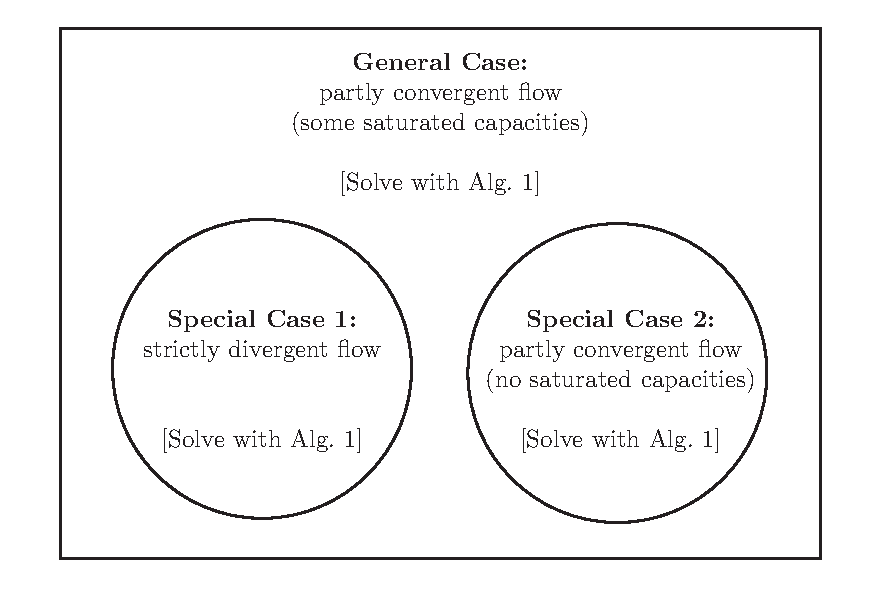
\includegraphics[width=\textwidth]{images/cases}
  \caption{Graphical illustration of problem cases}
  \label{fig:cases}
\end{figure}

We present a mathematical formulation for the special case. First, we present four additional parameter definitions

\begin{align*}
\Phi_o &\colonequals  \text{set of extreme agent feasible solutions for output $o \in O$}\\
%\gamma_{\theta,o} &\colonequals \text{quantity of output $o \in O$ produce by the principal solution $\theta \in \Theta$}\\
\alpha_{\phi_o,r} &\colonequals \text{quantity of resource $r \in R$ consumed by the agent solution $\phi_o \in \Phi_o$}\\
\delta_{\phi_o,o} &\colonequals \text{quantity of output $o \in O$ consumed by the agent solution $\phi_o \in \Phi_o$}\\
g_{\phi_o} &\colonequals \text{value of solution $\phi_o \in \Phi_o$ for the agent}\\
\intertext{and four additional variable definitions}
y_{\phi_o} &\colonequals \text{proportion of the final agent solution built from agent solution $\phi_o \in \Phi_o$}\\
\sigma_{\phi_o} &\colonequals \text{dual price of limit $o \in O$ for agent solution $\phi_o \in \Phi_o$} \\
\mu_{\phi_o} &\colonequals \text{dual price of output $o \in O$ for agent solution $\phi_o \in \Phi_o$}\\
\pi_r &\colonequals \text{dual price of resource $r \in R$}\\
\end{align*}

We can now formulate the special case of the agent's optimization problem as follows, decomposing the general case problem into output-wise subproblems.

\begin{align} 
  \intertext{The primal formulation of the agent's optimization problem is}
    z_A(x) \colonequals \boldsymbol{\max} \sum_{o \in O} \sum_{\phi_o \in \Phi_o} g_{\phi_o} y_{\phi_o} \\
    \shortintertext{\textbf{subject to} \nonumber} \\
    \sum_{o \in O} \sum_{\phi_o \in \Phi_o} \alpha_{\phi_o,r} y_{\phi_o} & \leq u_r , & \forall r \in R \\
    \sum_{\phi_o \in \Phi_o} \delta_{\phi_o,o} y_{\phi_o} & \leq 1 , & \forall o \in O \\
    \sum_{\phi_o \in \Phi_o} y_{\phi_o} & \leq d_o = \sum_{\theta \in \Theta} \gamma_{\theta,o} x_{\theta} , & \forall o \in O \\
    \sum_{\theta \in \Theta} x_\theta & = 1 \\
    \sum_{\phi_o \in \Phi_o} y_\phi & = 1, & \forall o \in O\\
    y & \geq 0\\
    \intertext{The dual formulation of the agent's optimization problem is}
   z_A(x) \colonequals \boldsymbol{\min} \sum_{r \in R} u_r \pi_r + \sum_{o \in O} d_o \mu_o \\
    \shortintertext{\textbf{subject to} \nonumber} \\
    \sum_{r \in R} \alpha_{\phi,r} \pi_r + \sum_{o \in O} \delta_{\phi,o} \mu_o & \geq  g_{\phi} , & \forall \phi \in \Phi \\
    \pi, \mu & \geq 0 
\end{align}

Similarly to the general case, we can derive a bilevel problem formulation that is stable for both the principal and the agent, by requiring equality on the output consumption constraint.

\begin{align} 
    z_A(x) \colonequals \boldsymbol{\max}  \sum_{o \in O} \sum_{\phi_o \in \Phi_o} g_{\phi_o} y_{\phi_o} \\
    \shortintertext{\textbf{subject to} \nonumber} \\
    \sum_{o \in O} \sum_{\phi_o \in \Phi_o} \alpha_{\phi_o,r} y_{\phi_o}  - s_r  & = u_r, & \forall r \in R \\
    \sum_{\phi_o \in \Phi_o} \delta_{\phi_o,o} y_{\phi_o} & = \sum_{\theta \in \Theta} \gamma_{\theta,o} x_{\theta} , & \forall o \in O \\
    \sum_{o \in O} \sum_{r \in R} \alpha_{\phi_o,r} \pi_r + \sum_{o \in O} \delta_{\phi_o,o} \mu_o - \sigma_{\phi_o}  & = g_{\phi_o} , & \forall o \in O, \phi_o \in \Phi_o \\
    s_r \pi_r & = 0 , & \forall r \in R \\
    \sigma_{\phi_o} y_{\phi_o} & = 0 , & \forall \phi_o \in \Phi_o \\
    \sum_{\theta \in \Theta} x_\theta & = 1 \\
    \sum_{\phi_o \in \Phi_o} y_{\phi_o} & = 1 & \forall o \in O \\
    y, \pi, \mu & \geq 0 
\end{align}

We can formulate the principal's optimization problem by modifying the objective function to express the sum of principal and agent solution values, from the perspective of the principal.

\begin{equation} 
    z_A(x) \colonequals \boldsymbol{\max} \sum_{o \in O} \sum_{\theta \in \Theta} v_{\theta} x_{\theta} + \sum_{\phi_o \in \Phi_o} w_{\phi_o} y_{\phi_o} \\
\end{equation} 
\begin{align} 
    \shortintertext{\textbf{subject to} \nonumber} \\
    \sum_{o \in O} \sum_{\phi_o \in \Phi_o} \alpha_{\phi_o,r} y_{\phi_o}  - s_r  & = u_r, & \forall r \in R \\
    \sum_{\phi_o \in \Phi_o} \delta_{\phi_o,o} y_{\phi_o} & = \sum_{\theta \in \Theta} \gamma_{\theta,o} x_{\theta} , & \forall o \in O \\
    \sum_{o \in O} \sum_{r \in R} \alpha_{\phi_o,r} \pi_r + \sum_{o \in O} \delta_{\phi_o,o} \mu_o - \sigma_{\phi_o}  & = g_{\phi_o} , & \forall o \in O, \phi_o \in \Phi_o \\
    s_r \pi_r & = 0 , & \forall r \in R \\
    \sigma_{\phi_o} y_{\phi_o} & = 0 , & \forall \phi_o \in \Phi_o \\
    \sum_{\theta \in \Theta} x_\theta & = 1 \\
    \sum_{\phi_o \in \Phi_o} y_{\phi_o} & = 1 & \forall o \in O \\
    y, \pi, \mu & \geq 0 
\end{align}


\section{Solution Methodology}

We originally set out to design an iterative solution methodology for the general case, based on the pioneering work of \citet{fortuny1981representation} and \citet{bard1982explicit}, however convexity issues limited this approach to local optimal solutions. 
Consequently, we decided to focus our algorithmic development efforts on special cases which we could solve to global optimality.

By limiting the problem domain to the special cases, we eliminate the possibility of interaction between outputs $o \in O$.
The optimal solution to the lower-level problem can then be described as the sum of optimal solutions to output-wise sub-problems.  
This property allows us to compute output-wise upper bounds on agent consumption behaviour.
These upper bounds can subsequently be used to optimally constrain the upper-level problem.
This is the basis of our solution methodology for the special case.
Algorithm \ref{alg:bilevel_specialcase} describes the solution methodology using pseudo-code.

\vspace{12pt}
\begin{algorithm}[H]
  \DontPrintSemicolon
  \SetKwInOut{Output}{Output}
  \Output{Global optimal wood supply solution $x^*$}
  \BlankLine
  \ForEach{output $o \in O$} {
    Determine upper bound $u_o = z_P^o$ on agent consumption of output $o$ (i.e., solve integrated sub-problem with all non-targeted outputs disabled). \;
  }
  \ForEach{output $o \in O$} {
    Set upper bound constraint $\gamma_o \leq u_o$ on quantity of output $o$ produced by the upper level of the integrated master problem. \;
  }
  Solve integrated master problem. \;
  \caption{Bilevel model solution algorithm (special case: no saturated joint capacity constraints)}
  \label{alg:bilevel_specialcase}
\end{algorithm}
\vspace{12pt}

Algorithm \ref{alg:bilevel_generalcase} describes an algorithm to solve the general case to global optimality by simple enumeration (i.e., iterate over the set of all possible convex subproblems, and return the best solution). Algorithm 2 is of limited practical interest, as computational effort required to solve realistically-sized instances by enumeration would be prohibitive. Efficiency of the general algorithm could potentially be improved by replacing subproblem enumeration with a custom branching algorithm taking advantage of problem structure, however we have not tested this approach.

\vspace{12pt}
\begin{algorithm}[H]
  \DontPrintSemicolon
  \SetKwInOut{Output}{Output}
  \Output{Global optimal wood supply solution $x^*$}
  \BlankLine
  \ForEach{output $o \in O$}{
    Generate subproblem (isolate output $o$ in lower-level problem). \;
    Solve subproblem. \;
    }
  Sum subproblem solutions. \;
  Build super-saturated process set $P_s$ (i.e., find violated capacity constraints). \;
  \ForEach{combination of super-saturated process $p \in P_s$ and output $o \in O$} {
    Generate subproblem (restrict certain combinations of output $o$ and process $p$). \;
    Solve subproblem. \;
    \If{subproblem feasible (i.e., no violated capacity constraint)} {
        Add solution $x$ to feasible solution set $X$. \;
    }
  }
  \Return{Global optimal solution $x^*$ (i.e., best solution in feasible set $X$).} \;
  \caption{Bilevel model solution algorithm (general case: saturated joint capacity constraints)}
  \label{alg:bilevel_generalcase}
\end{algorithm}
\vspace{12pt}

The bilevel model can be solved to global optimality with relative ease when lower level input datasets have some special properties. 
The test dataset used in our test simulations corresponds to special case 2.
Special case 1 occurs if the product lines (i.e., outputs $o \in O$) in the lower level model are totally independent (i.e., strictly divergent). 
Before elaborating further on this condition, we will describe the lower level data model in a bit more detail.

The lower level data model can be described as a network of abstract processors connected by product flows.
Figure \ref{fig:abstract_process} presents a graphical representation of an abstract processor node.
An abstract process consumes inputs and resources, and produces outputs.

\begin{figure}[h]
  \centering
  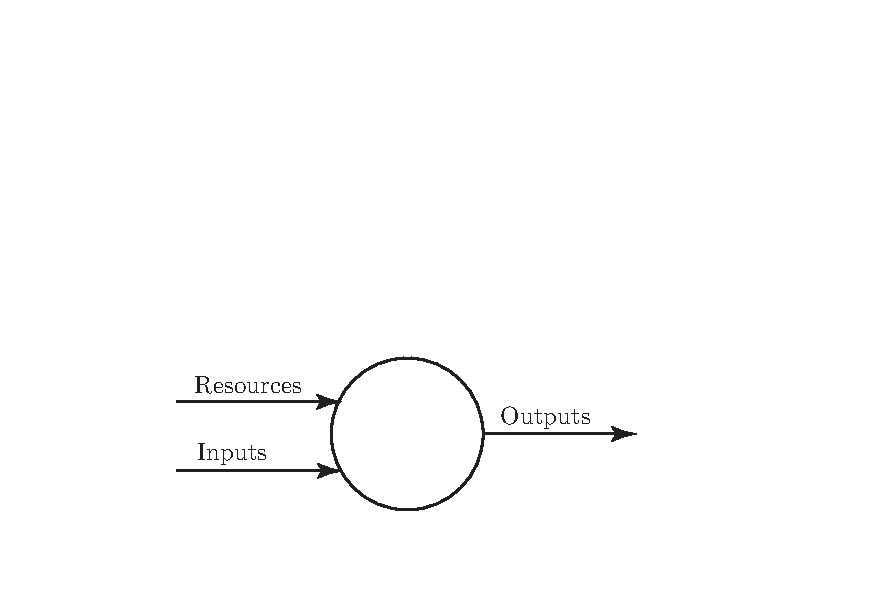
\includegraphics[width=70mm]{images/abstract_process}
  \caption{Graphical representation of an abstract process}
  \label{fig:abstract_process}
\end{figure}
 
At the upstream (source) end of this network is the interface between upper and lower level models. 
Output from the first planning period in the upper level model (i.e., outputs $o \in O$) becomes input material that can be transformed by the lower-level network. 
At the downstream (sink) end of the lower level network, external clients are willing to pay set unit prices to satisfy a bounded demand for each end product. 
This end client demand enables the model to generate profits by pulling a subset of available fibre supply through the network to satisfy a (profit-maximizing) subset of end client demand.
When raw upper-level model outputs are first pulled into the lower network, they must go through one of several front-line processor nodes that convert the raw wood supply into species-wise assortments of logs. 
These front-line processors simulate the interface between the forest and the mills (i.e., the process of harvesting and delivering logs to mills, including transportation cost, which can vary depending on the forest zone from which the raw volume inventory was picked).

Raw upper-level volume is classified by species, and this species-wise distinction may (optionally) be maintained as the outputs are pulled into the lower-level network, depending on configuration of front-line processors. 
For example, in the case of our test dataset, the front-line processors are configured to convert raw upper-level volume into assortments of either hardwood or softwood logs of various sizes \footnote{Our upper-level dataset uses a more fine-grained classification of tree species, which is aggregated into \emph{hardwood} and \emph{softwood} log types by the front-line processors.}.

Due to the abstract nature of the lower-level processor implementation, it is possible to simulate any combination of divergent and convergent product flows. 
Strictly divergent networks correspond to special case 1, and can be solved to global optimality using Algorithm \ref{alg:bilevel_specialcase}. 
Special case 2 occurs when the network includes convergent product flows, but no joint capacity constraints are saturated. 
Although somewhat more difficult to detect, special case 2 is not problematic and can also be solved to global optimality using Algorithm \ref{alg:bilevel_specialcase}.
For special cases 1 and 2, each product line $o \in O$ can be treated as an independent subproblem. 
The optimal value of $z_{A_o} (x)$ for output $o$ is equal to $\argmax_{v_o} p(v_o)$, where $p(v_o)$ is a concave function describing profit for any non-negative consumption volume $v_o$ (see Figure \ref{fig:pvo}). 
%This corresponds to the maximum volume that the agent can be expected to consume for a given product line $o$, which we use as an upper bound on harvest level for product line $o$ in the final step of Algorithm \ref{alg:bilevel_specialcase}. 

\begin{figure}[h]
  \centering
  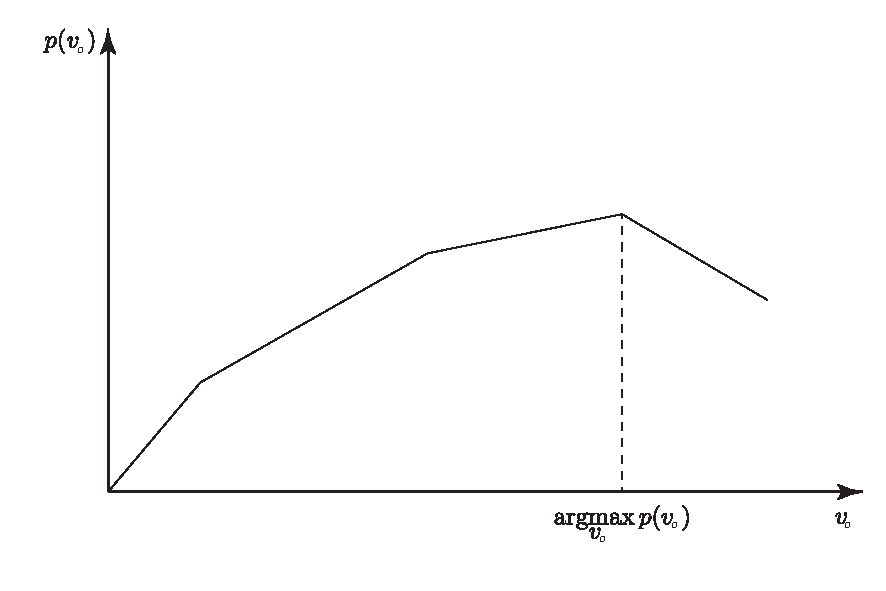
\includegraphics[width=\textwidth]{images/pvo}
  \caption{Illustration of concave profit function of a hypothetical product $o$}
  \label{fig:pvo}
\end{figure}

%For special cases 1 and 2, the profit functions are implicitly embedded in the dataset. 
The product-wise subproblems can be represented using the lower-level model by disabling all non-targeted outputs\footnote{Non-targeted outputs can be disabled by manipulating input parameters of the upper level model, setting conversion efficiency and conversion cost of front-line processors to null values. Instead of converting wood supply units to log assortments, the modified front-line processors now consume all non-targeted outputs at zero cost, which blocks non-targeted outputs from further flow through the lower-level model network.}. 
We can then easily solve each subproblem to obtain the optimal sub-problem solutions without having to explicitly locate intermediate inflection points of profit function $p(v_o)$. 
This corresponds to the maximum volume that the agent can be expected to consume for a given output $o$, which we use as an upper bound on harvest level for output $o$ in the final step of Algorithm \ref{alg:bilevel_specialcase}.

Note that output from our bilevel model is structurally identical to output from the classic model (i.e., output-wise upper bounds on harvest levels, bundled with required levels of pre-commercial sylviculture treatments). 
Thus, our bilvel model can potentially be used as a drop-in replacement for the single level model.
\todo{Is this really not clear?}
%We test this using a case study, which we describe in the next section.

%\section{Computational Experiment}
\section{Materials and Methods}

This section describes the computational experiments we conducted to compare performance of classic and bilevel wood supply models.

\subsection{Description of Dataset}

We tested our bilevel solution methodology on a realistic synthetic dataset from Quebec, Canada.
The study area is a forest management unit (FMU 031-53) located in the boreal forest region of the province of Quebec, Canada. It covers an area of approximately 102 040 hectares. 
%The forest inventory data for this area was compiled into a number of management strata for the purposes of wood supply modeling.  
Approximately (88\%) of initial growing stock is from softwood species, with the remaining (12\%) of initial growing stock in hardwood species. 
Although some pure softwood stands are present, forest cover is dominated by mixed-wood stands containing different proportions of
hardwood mixed in with the softwood. See \citet{paradis2013risk} for a more detailed description of the study area.

Output from the upper-level (forest) model is aggregated into two outputs: \emph{softwood} and \emph{hardwood}. 
The lower-level (industrial) model has limited capacity for transforming hardwood (approximately $1/3$ of potential sustainable wood supply). 
%The upper level model has a single (clearcut) harvest treatment implemented, which has the effect of ``bundling'' hardwood and softwood together in the upper-level model solution.
%A combination of limited hardwood processing capacity in the lower level and output bundling in the upper level indirectly constrains softwood consumption in the lower level.
The classic wood supply model therefore systematically over-estimates short-term hardwood fibre consumption.

% We have not thus far succeeded in developing a solution methodology that guarantees convergence on global optimality for the general convergent case with saturated capacity constraints 
% However, we have developed an iterative solution methodology that we believe could converge on locally optimal solutions in a finite number of iterations. 
% Our methodology for the general case relies on iterative shadow price feedback from the lower level to guide selection of new columns to add to the basis in a column-generation--based algorithm embedded in the upper level. 
% We have not yet implemented or tested the solution methodology for the general case.

%See \citep{paradis2013risk} for a detailed description of case study dataset.  
We use the same test dataset as in \citet{paradis2013risk}, which is an instance of special case 2. Although chip flows from both hardwood and softwood sawmills converge at the pulp mill, we have determined empirically that its capacity is sufficient to avoid saturation problems.

\subsection{Simulation Framework}

We use the two-phase rolling-horizon simulation framework developed by \citet{paradis2013risk} as a testbed in which to compare the long-term performance classic and bilevel wood supply model formulations. 
%This framework uses agency theory to model interaction between government wood supply planners (the \emph{principal} and industrial fibre consumers (the \emph{agent}.

% assumes that long-term AAC-maximizing wood supply planning is controlled by government planners (the \emph{principal}), and that short-term profit-maximizing fibre consumption is controlled by industry planners (the agent). 
The principal and the agent make their moves sequentially, in a two-phase game, repeated 30 times. The framework simulates forest growth between each 5-year rolling-horizon re-planning cycle. The principal has the advantage of the first move, which means he can set AAC to any level of his choosing. Thus, the simulation results presented here show the cumulative result of 150 years of iterative replanning, under different combinations of principal and agent behaviour. 

% We tested our bilevel model within the simulation framework presented in \citet{paradis2013risk}. This framework models the wood procurement planning cycle as a two-phase process, which allows us to simulate principal-agent interaction and simulate rolling the long-term planning horizon forward one period.


\subsection{Experimental Methodology}
\label{sec:experimental_methodology2}

We present six scenarios, showing impact of replacing the classic wood supply model with the bi-level wood supply model. Within any given scenario, simulation parameters for the industrial fibre consumption network\footnote{Mill capacities, costs, prices, client demand, etc.} are held constant for all 30 planning cycles. 
%Table X summarizes the key simulation parameters for each scenario. 

Scenario 1 simulates \emph{status quo} behaviour for both principal and agent, and acts as a control scenario. At each planning cycle, the principal maximizes even-flow AAC (30-period horizon) using the classic wood supply model, then the agent maximizes first-period profits (1-period horizon) by consuming the optimal subset of the wood supply offered by the principal. The principal does not consider the agent's fibre consumption capacity when determining AAC. 

Scenario 2 presents a perfect-implementation bilevel scenario; rather than being allowed to re-plan harvesting on a one-period horizon, the agent is forced to exactly implement the first period of the principal's bilevel wood supply solution. This scenario shows the best-case performance of the bilevel model solution, and is equivalent to the principal controlling the entire wood procurement process from stump to mill gate.

Scenario 3 is the basic bilevel scenario. The principal uses the bilevel model to determine AAC, and the agent is allowed to replan harvesting on a one-period horizon, choosing the profit-maximizing subset of available wood supply. Due to the optimal formulation of the bilevel model and perfect anticipation of volume consumption, the agent always chooses to harvest the entire wood supply. However, the agent may select to harvest this volume from a different combination of forest types than what was prescribed in the first period of the principal's optimal solution. This reflects the distributed nature of forest management planning on Crown land in many jurisdictions.

The contrast between scenario 1 and scenario 2 shows the sensitivity of long-term wood supply to deviations from the principal's optimal wood supply plan.

Scenarios 4 and 5 simulate reducing the softwood supply allocated to the agent to 80\% and 60\% of AAC. Adjusting AAC allocation indirectly creates a buffer stock to protect against decreases in wood supply induced by agent harvest re-planning (i.e., compensation for the principal's incomplete control of the fibre procurement process).

Scenario 6 shows the effect of simulating centralized agent fibre procurement planning on long-term wood supply. For this scenario, we relax the agent's line-wise profitability contraint, and allow him to maximize total network profit. For this scenario, we allow any overflow fibre (hardwood, in our case) to be disposed of at a moderate unit cost. This allows the agent's softwood line to subsidize the disposal of excess hardwood from harvesting of mixed-wood stands, thereby increasing the agent's total potential fibre consumption. This in turn relaxes the lower-level consumption constraints in the principal's bilevel model, thereby allowing him to increase the wood supply offer without compromising long-term sustainability. 

%Scenarios 2 through 6 replace the classic wood supply model with with bilevel model. These scenarios show the long-term cumulative impact of anticipating industrial fibre consumption behaviour within the AAC-determination process. 

%Scenarios 1, 3, 4 and 5 simulate standard agent behaviour; the agent is allowed to select any available forest units for harvesting in the first period, subject to species-wise AAC upper-bound constraints. The agent harvests the entire wood supply for both species groups. This is expected behaviour, given that we simulate perfect anticipation of agent behaviour (i.e., we use the same optimization model formulation for both the agent-anticipation constraint embedded into the bilevel model, and for simulation of agent consumption behaviour in the second phase of the rolling-horizon replanning simulation, as in \citet{paradis2014bilevel}. Note that although the the anticipation mechanism embedded into the bilevel model perfectly anticipate the \emph{volume} of fibre consumption, these may be harvested from different forest units than than the ones that make up the basis of the first period of principal's optimal wood supply solution. This reflects the distributed nature of forest management planning on Crown land.

%Scenario 2 forces the agent to exactly implement the principal's first-period optimal solution. This is an optimistic scenario, to illustrate the best-case performance of the bilevel model solution.


% We present a computational experiment using two scenarios (control and test). 
% The purpose of the computational experiment is to show convergence of our solution methodology, and to compare solution times (i.e., computational effort) between control and test scenarios.

% The \emph{control} scenario corresponds to the \emph{status quo} (i.e., our best attempt at simulating current principal and agent behaviour).
% The \emph{test} scenario uses the bilevel model (instead of the classic model) to simulate the principal's behaviour in the first stage of each planning cycle; all other parameters are held constant. 
% %The purpose of the computational experiment is to show that our solution methodology for the special case of the bilevel problem converges quickly on a globally optimal solution, using a dataset of realistic size and complexity.

% For each planning cycle, principal and agent each get to make their move sequentially. 
% First the principal maximizes even-flow wood supply (30-period horizon), then the agent maximizes first-period profits (1-period horizon).
% %Planning horizon length is 30 periods for the first (principal) phase, and 1 period for the second (agent) phase.  
% Planning period length is 5 years.
% The test scenarios presented in this paper show results from a single two-phase planning cycle.

% Note that we simulate \emph{perfect} anticipation of agent behaviour, by using identical model formulations for both the agent-anticipation mechanism (in the first phase of the simulation) and the agent-execution mechanism (in the second phase of the simulation).
% This helps clearly illustrate convergence of the solution methodology under best-case conditions.

% %We present results from a single cycle of the two-phase wood supply planning problem (i.e., principal determines sustainable wood supply, agent consumes profit-maximizing subset of the wood supply).  

% %Long-term effect of the bilevel formulation, after repeated planning cycles, will be presented in a future publication. 


\section{Results}
\label{sec:results2}

We present experimental results in two stages. First, we show detailed results comparing output from the first planning cycle of scenarios 1 and 2. Next, we show result of simulating 30 rolling-horizon planning cycles for scenarios 1 to 6.

Figure \ref{fig:scenarios_detail} presents detailed results from the first planning cycle of scenarios 1 (control) and 3 (bilevel).
 
For the control scenario, potential hardwood fibre supply is 64\,583\,\si{\cubic\metre}, whereas actual consumption is only 20\,800\,\si{\cubic\metre}.
The difference between planned and executed hardwood fibre consumption volumes is due to the limited processing capacity at the (single) hardwood sawmill in the lower-level model.
The entire softwood fibre supply is consumed by the agent, as we would expect, as both end-product demand and processing capacity for the softwood line are high enough to accommodate more softwood fibre than the forest can supply. 
This phenomenon (of consuming certain components of the wood supply entirely while other components are only partially consumed) can be observed to varying extents in practice, where processing capacity and market demand are often misaligned with the proposed wood supply.

In order to harvest the full softwood supply volume while only harvesting a third of the hardwood supply, the agent must favour forest stands that have a high proportion of softwood (low proportion of hardwood).
The wood supply model is sensitive to deviation from the timing and location of harvesting activities prescribed in the first period of the optimal solution.
Even slight deviations from the optimal solution carry a high risk of rendering the solution infeasible (from the perspective of the principal, in the form of wood supply shortages) in future periods.   
This is inherently problematic, as the optimal solutions from wood supply models were never intended to be implemented as-is\footnote{Intended usage of wood supply model solutions is limited to estimating species-wise upper bounds on short-term timber licence allocations, such that long-term sustainability of the wood supply is not irreversibly compromised.
Producing an operationally feasible fibre procurement plan (including access road construction and maintenance, harvesting, transportation, and follow-up silviculture treatments) from the first period of the wood supply plan requires considerable dis-aggregation and refinement.}.

%\footnote{Wood supply modelling is considered a long-term planning exercise. Consequently, wood supply models are highly simplified representations of the complex interactions between forest growth and anthropogenic disturbances (i.e., harvesting). Input data is highly aggregated.}

Thus, minimizing the gap between planned and executed harvesting volume should help reduce the risk of future wood supply failures.
The primary motivation for developing the bilevel model formulation presented here is to proactively mitigate selective wood supply consumption behaviour. 
We implement this idea by embedding explicit anticipation of industrial fibre consumption into the wood supply model, such that the principal offers the maximal sustainable wood supply that will be entirely consumed by the agent. 
Re-defining the wood supply problem in this way improves the quality of linkage between strategic and tactical planning levels.

%Although the upper-level wood supply model uses a 30-period horizon to predict future wood supply, these model are typically used on a 1-period rolling-horizon (i.e., the model is re-run at the beginning of each planning period). 

Results show that our bilevel anticipation mechanism completely eliminates over-estimation of hardwood fibre consumption volume. 
Fibre consumption by the agent is exactly equal to wood supply volumes offered by the principal (20\,800\,\si{\cubic\metre} for hardwood, and 323\,759\,\si{\cubic\metre} for softwood ).
This is the desired outcome from the bilevel model, and represents a global optimal solution for this instance. Note that the agent plans his own harvesting in the second stage of the planning cycle (using his single-period profit-maximizing model), so harvest areas will not typically match the first period of the principal's plan, even if harvest volume is exactly equal.  
%, given that our test dataset is an instance of special case 2 (i.e., convergent network with non-saturated shared resource). 

\begin{figure}[H]
  \centering
  \medskip
  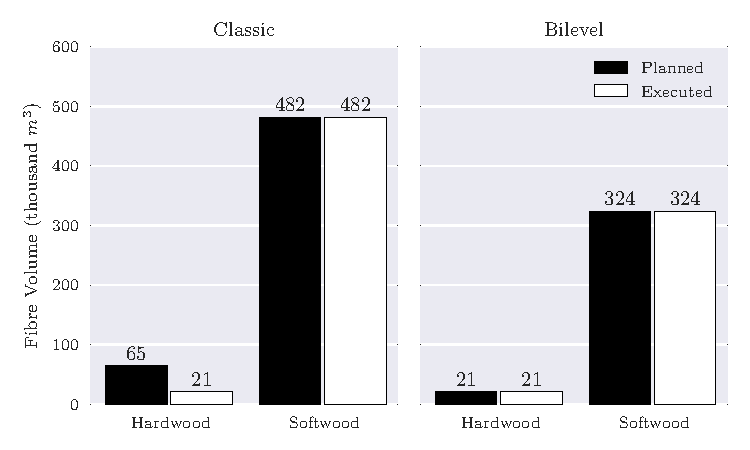
\includegraphics[width=\textwidth]{images/article2_compbar}
  \caption{Comparison of planned and executed volumes}
  \label{fig:scenarios_detail}
\end{figure}

Table \ref{tab:scenarios} presents intermediate results from each step of the bilevel solution method (see Algorithm \ref{alg:bilevel_specialcase}).
We present this data to show how we derive the optimal upper bounds to the wood supply problem from solutions to output-wise sub-problems.
Hardwood consumption capacity (20\,800\,\si{\cubic\metre}) is the binding constraint in this case. 
Our anticipation mechanism shows that the softwood line could have profitably consumed up to 584\,861\,\si{\cubic\metre} of softwood in the first planning period, however the species-wise even-flow constraints on the upper-level wood supply model limit long-term softwood harvest level to 323\,759\,\si{\cubic\metre}.
As expected, the agent's fibre consumption volume in the second phase of the simulation is exactly equal to the wood supply.
This shows that the bilevel model eliminates the gap between planned and executed fibre consumption levels, thereby fulfilling its intended purpose.

\begin{table}
\caption{Bilevel solution method Intermediate results}
\label{tab:scenarios}
\renewcommand{\tabcolsep}{2pt}
\begin{tabular}{llrr}
\toprule 
Phase & Description & \multicolumn{2}{c}{Volume (\si{\cubic\metre})} \tabularnewline
&& Hardwood & Softwood \tabularnewline
\midrule
1 (principal) & Upper bound on \emph{hardwood} consumption & 20\,800 & - \tabularnewline
1 (principal) & Upper bound on \emph{softwood} consumption & - & 584\,861 \tabularnewline
1 (principal) & Maximum even-flow wood supply levels & 20\,800 & 323\,759 \tabularnewline
2 (agent) & Agent fibre consumption & 20\,800 & 323\,759 \tabularnewline
\bottomrule
\end{tabular}
\end{table}

The classic model can be solved in a single step.
This corresponds to approximately 13 seconds of CPU time to solve classic wood supply model for the first (of 30) planning cycle in scenario 1.
For scenario 2, the bilevel model requires $\left|O\right| + 1$ steps to solve.
This corresponds to approximately $(4 + 6) + 10$ seconds of CPU time using our test setup.
We ran our tests on an Intel\textsuperscript{\textregistered} Xeon\textsuperscript{\textregistered} E5-2670 processor (20\,\si{\mega\byte} cache, 2.60 \si{\giga\hertz}).

Figures \ref{fig:scenarios} shows simulation results the six scenarios described in the previous section. For each scenario, Figure \ref{fig:scenarios}(a) plots species-wise AAC and fibre consumption for each of the 30 rolling-horizon re-planning cycles simulated. The same data are shown in Figure \ref{fig:scenarios}(b) using box-plots to illustrate the variability of period AAC and fibre consumption values across scenarios. The boxes encompass the inter-quartile range (IQR) with the median marked. The whiskers extend to $1.5 \text{IQR}$ past the closest quartile; any observations outside this range are marked as outliers using a dot symbol.


\begin{sidewaysfigure}%
  \centering
  \subfloat[][]{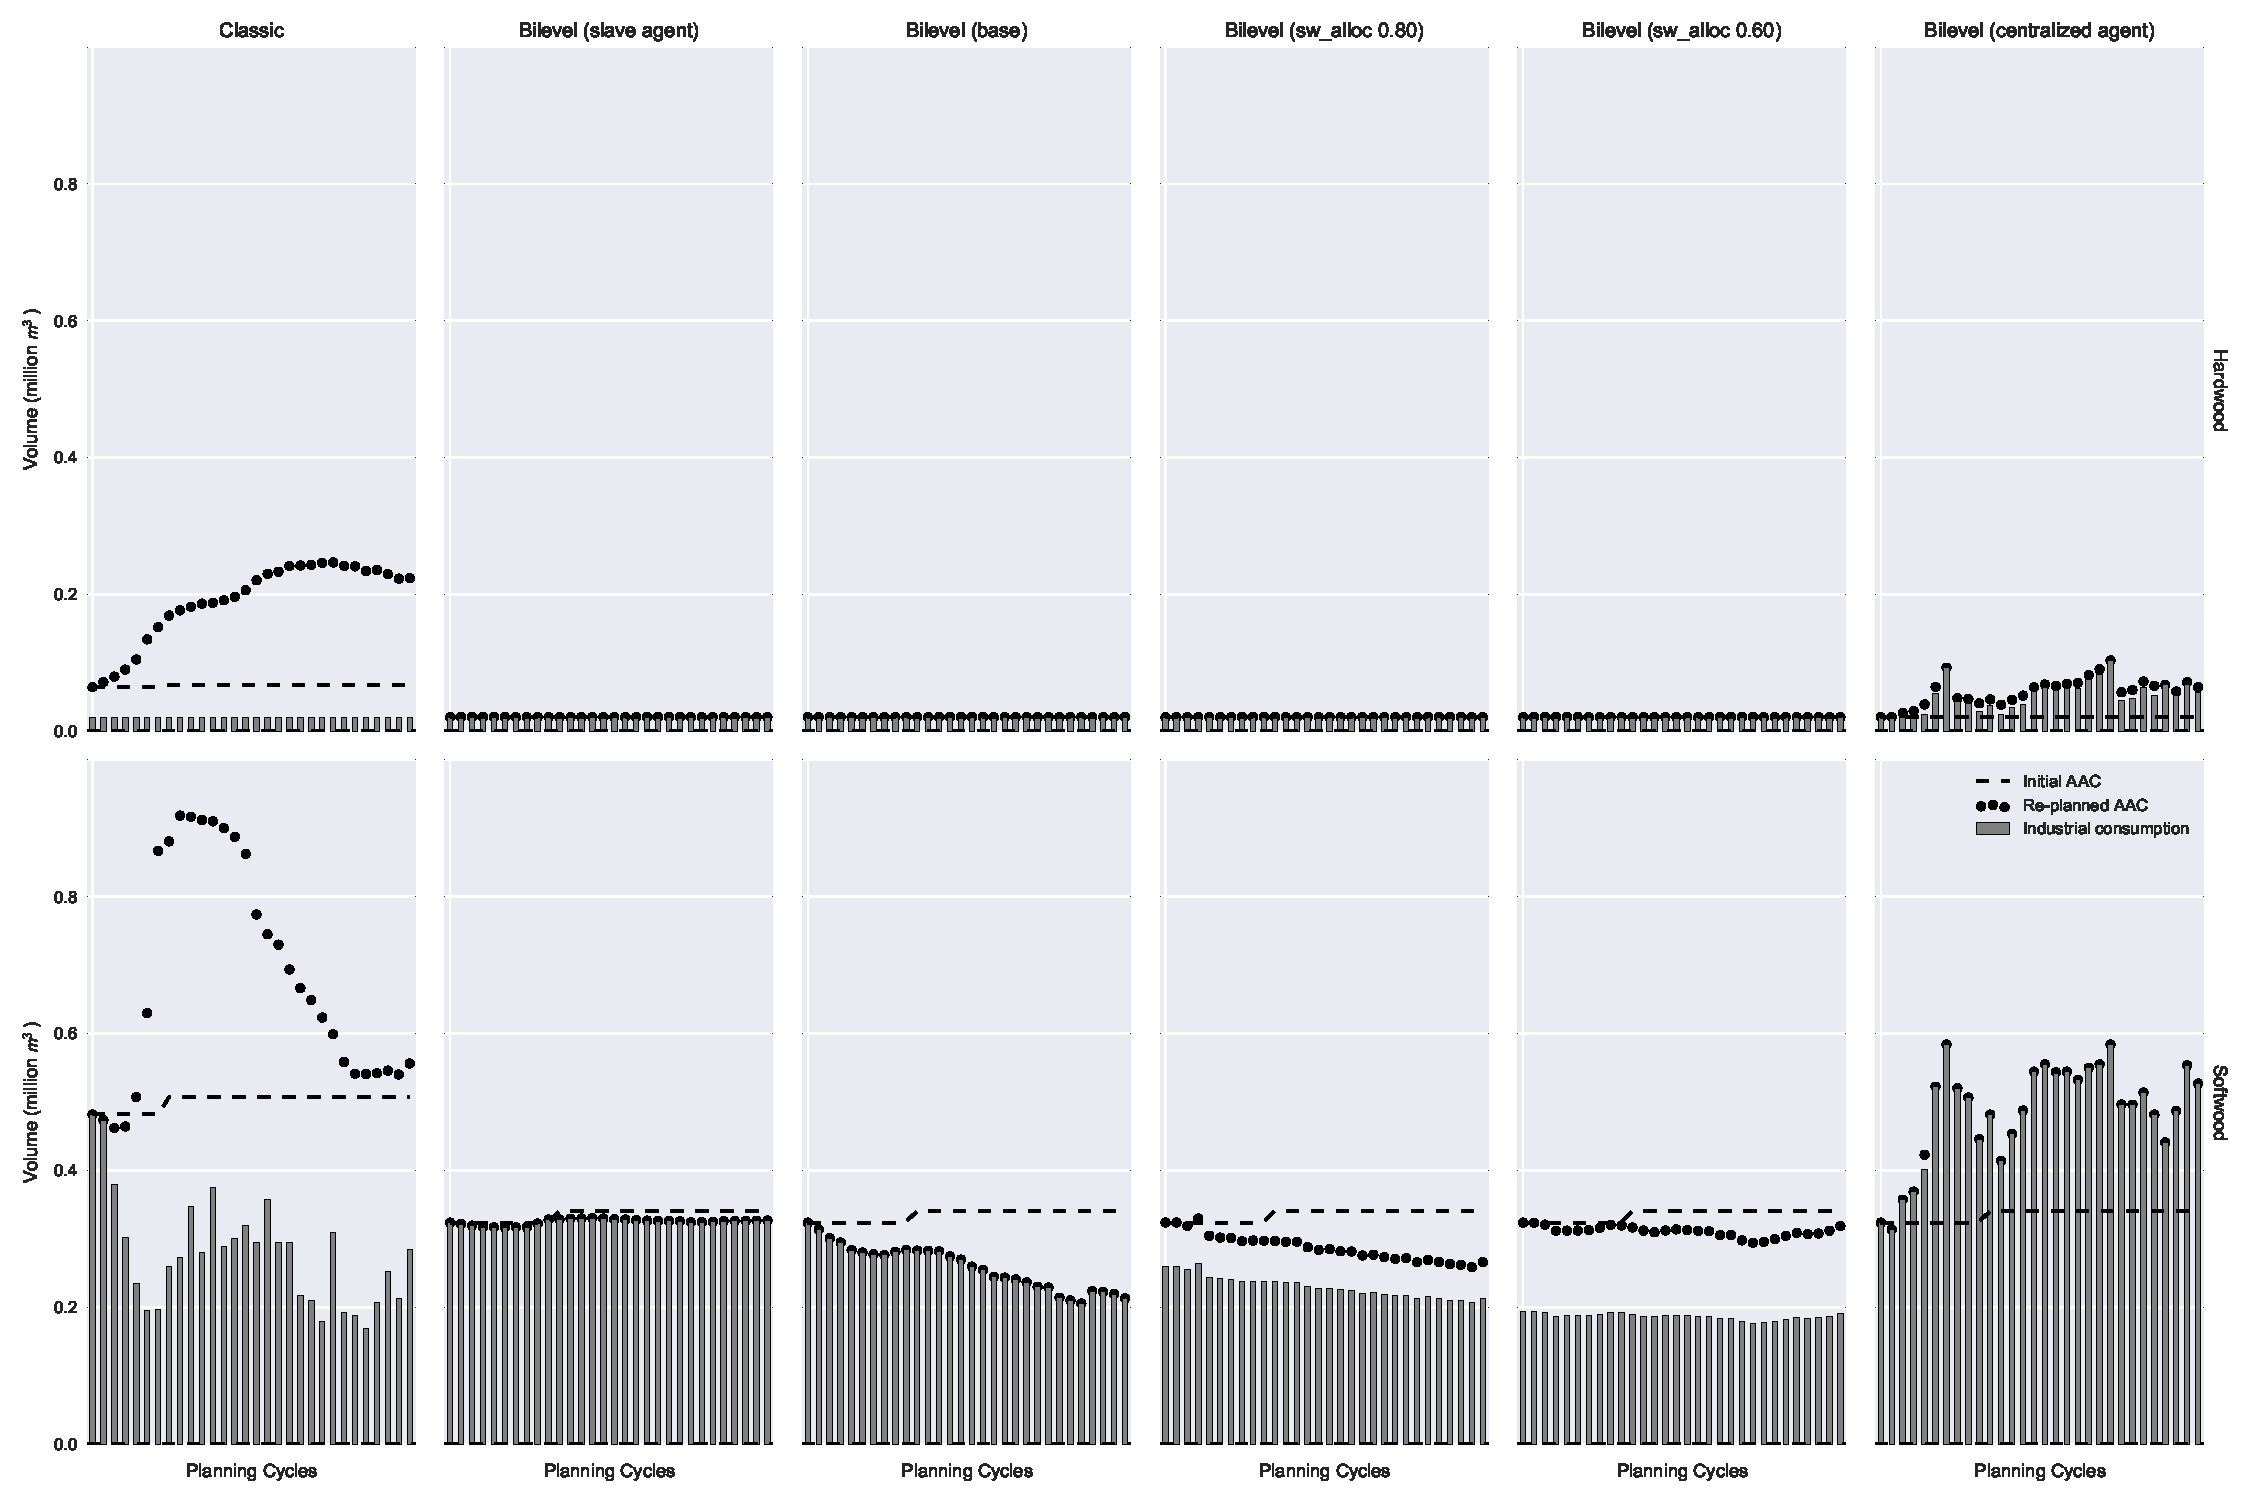
\includegraphics[width=\textwidth]{images/scenarios_timeseries}}%
  \caption{Species-wise AAC and fibre consumption for scenarios 1 to 6 (time series)}%
  \label{fig:scenarios}%
\end{sidewaysfigure}

\begin{sidewaysfigure}%
  \ContinuedFloat
  \centering
  \subfloat[][]{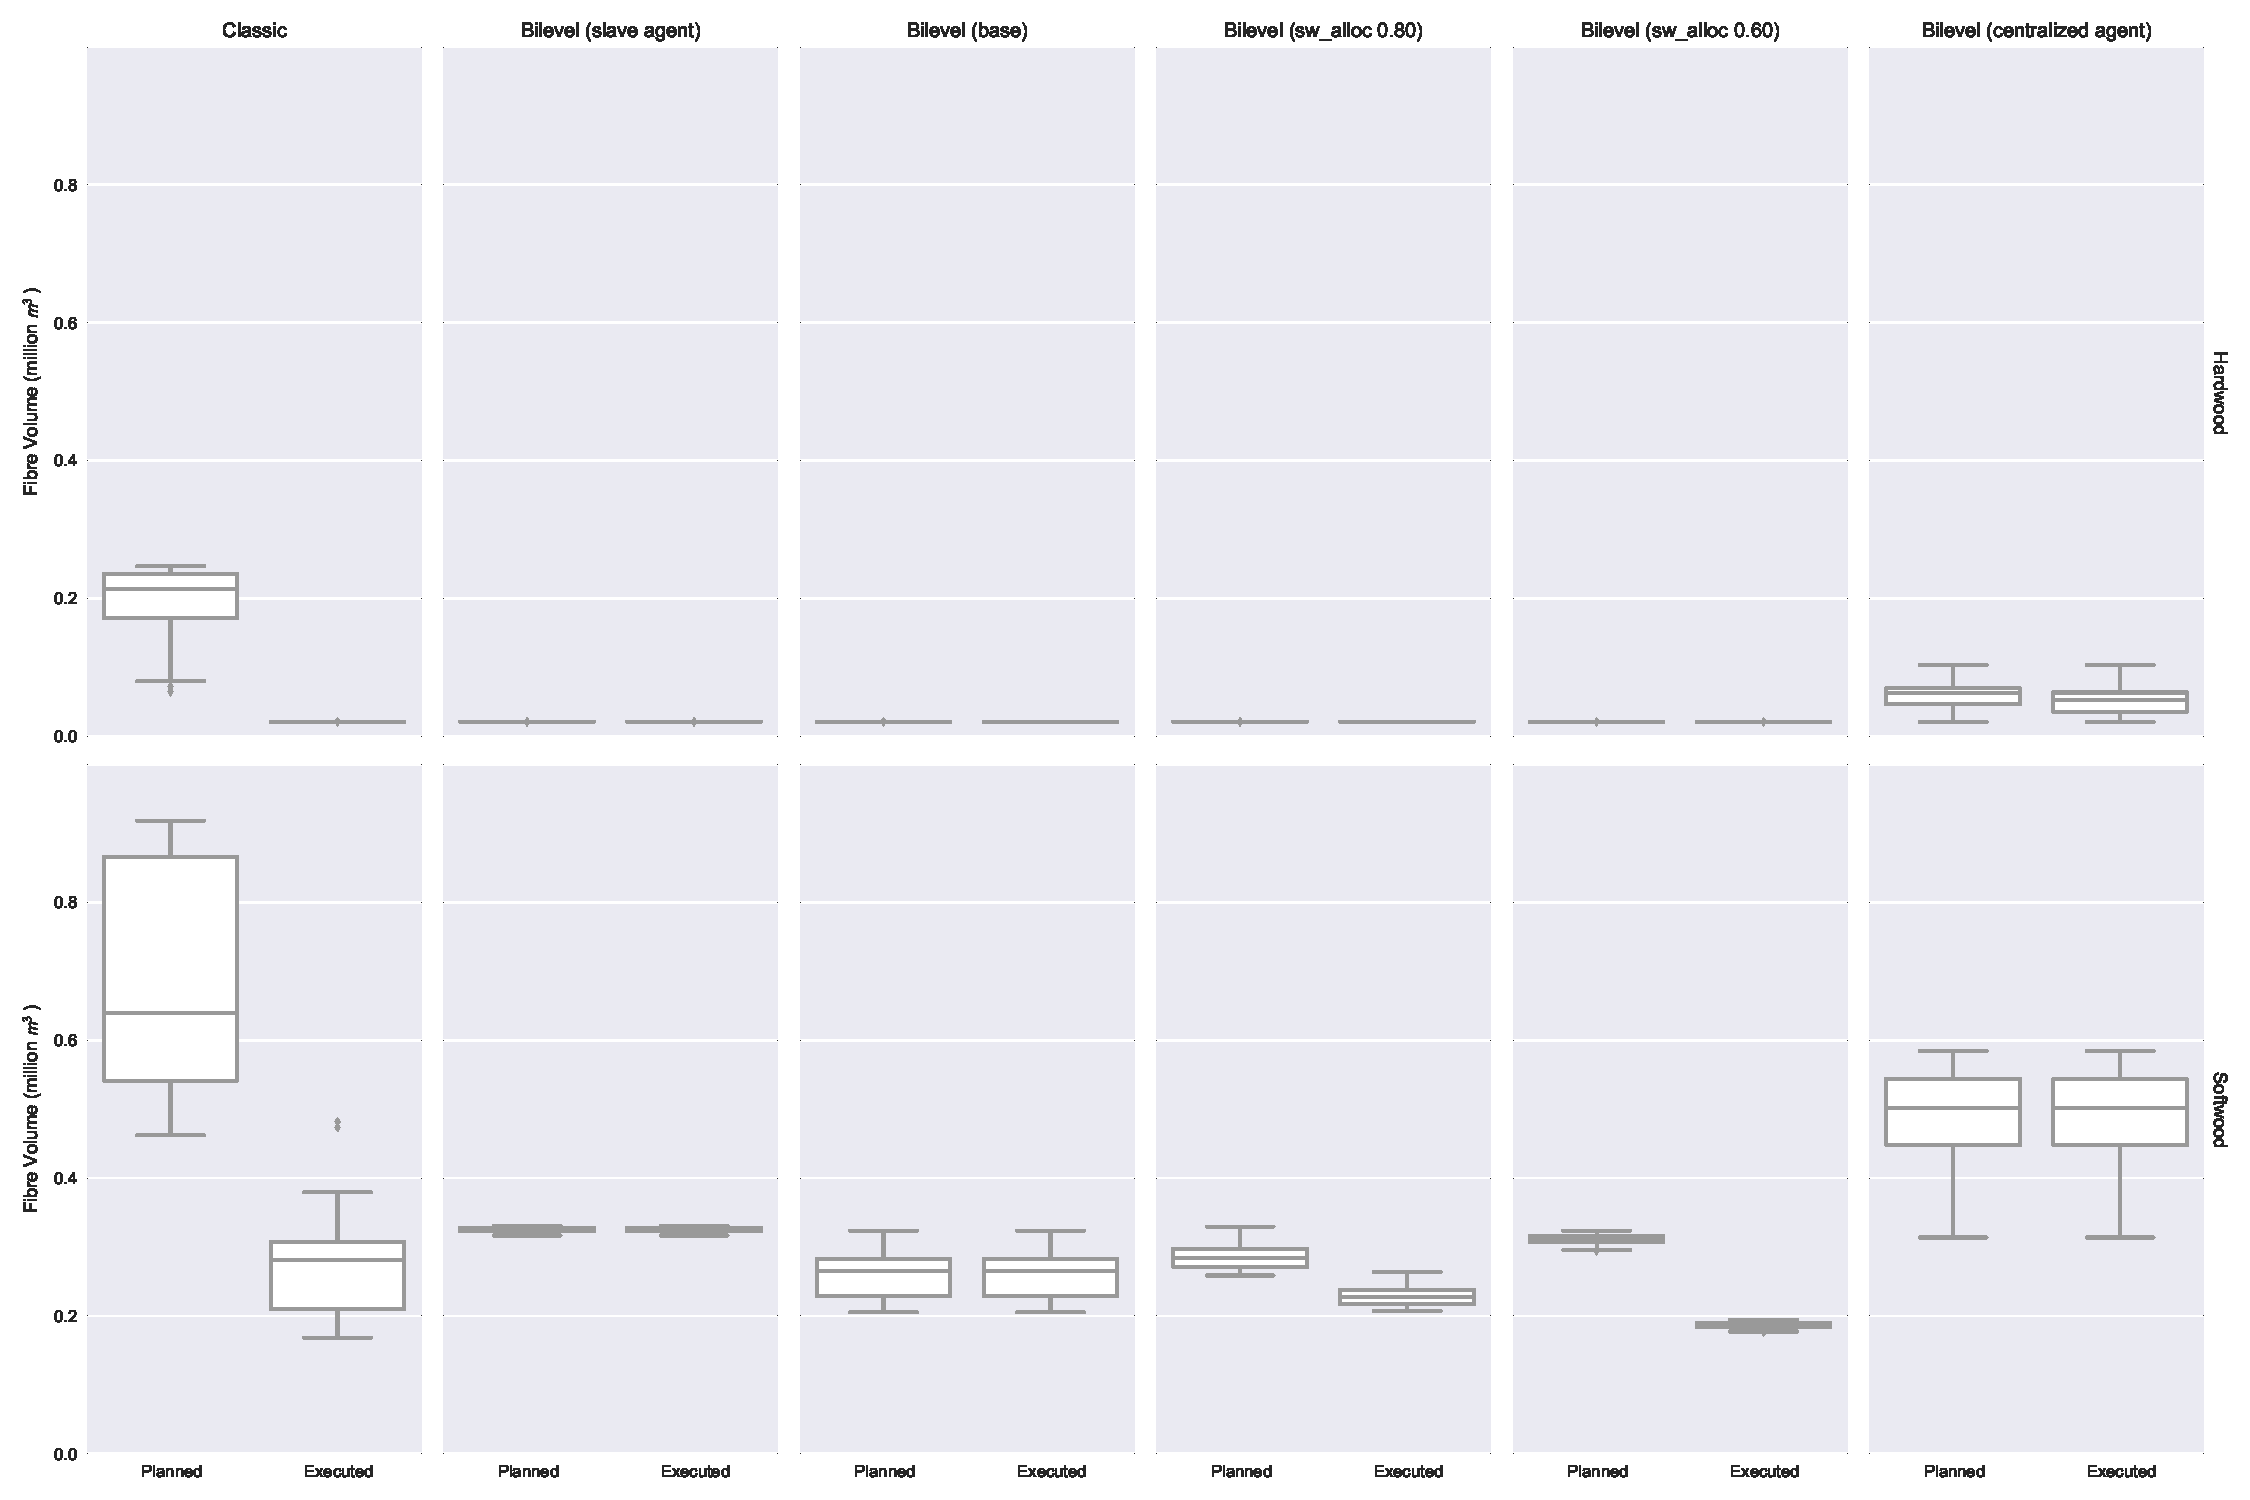
\includegraphics[width=\textwidth]{images/scenarios_boxplots}}%
  \caption{Species-wise AAC and fibre consumption for scenarios 1 to 6 (boxplots)}%
  %\label{fig:scenarios_plot}%
\end{sidewaysfigure}

%\begin{figure}%
%  \ContinuedFloat
%  \centering
%  \subfloat[][]{...figure code...}%
%  \caption[]{Species-wise AAC and fibre consumption for scenarios 1 to 6 (boxplots)}%
%  \label{fig:scenarios}%
%\end{figure}


\section{Discussion}
Scenario 1 shows the relative instability of the classic wood supply model. This is attributable to the species-skewed gap between AAC and fibre consumption volumes. Despite the harvest levels being systematically lower than AAC, the agent's preference for harvesting high-softwood-content stands gradually shifts the composition of the residual forest cover towards a higher hardwood content. \citet{paradis2013risk} use the term \emph{systematic drift effect} to describe this phenomenon.   

The principal uses the bilevel model to determine AAC for scenarios 2 through 6. By virtue of its formulation, the bilevel model completely eliminates the volume gap between AAC and fibre consumption. Note that we simulate perfect anticipation of agent fibre consumption \emph{volume}. For scenarios 3 through 6, we allow the agent to plan his own harvesting in the second phase of each planning cycle simulation; this explains the residual instability in long-term wood supply for scenarios 3 and 4.

Scenario 2 forces the agent to harvest the exact forest units that form the basis of the first period of the principal's optimal bilevel solution. The purpose of this scenario is to show that wood supply tracks almost perfectly along the initial bilevel AAC solution (even after 30 rolling-horizon re-planning cycles) under best-case conditions (i.e., when the principal controls wood procurement planning execution all the way to the mill gate). In practice, the decoupling point between the principal and the agent is not typically located this far downstream; scenarios 3 through 6 simulate a more conventional decoupling point.

Scenario 3 shows vastly improved stability (hence credibility) of the softwood supply levels, relative to the control scenario. Note the slight, but monotonic, downward trend of the softwood fibre supply for scenario 3. As discussed earlier, the contrast between scenarios 2 and 3 shows that the bilevel model is sensitive to even slight deviations the optimal wood supply model solution. This type of sensitivity to deviations from the optimal solution is typical of deterministic optimization models, as optimal solutions are invariably located along the boundary of the feasible region; even the slightest deviations from the optimal solution (or error in the constraint right-hand-side values) can induce problem infeasibility.

Scenarios 4 and 5 show the effect of reducing the proportion of AAC that is allocated to the agent, in an attempt to compensate for the residual drift seen in scenario 3. Reducing allocation is an indirect way for the principal to induce a buffer stock in the standing timber inventory. This tends to move the agent's solution away from the feasible boundary of the principal's solution space, thereby improving the robustness of the distributed wood supply planning process. Scenario 4 shows a marked reduction in drift compared with scenario 3. Residual drift is virtually eliminated in scenario 5, but at the expense of 40\% of the maximum potential (bilevel) sustainable wood supply. 

Intuitively, foregoing 40\% of the potential wood supply seems like a high price to pay to eliminate the residual drift in a bilevel modelling context. A more direct management approach to maintaining a buffer stock in standing timber inventory, as described in \citet{raulier2014increasing}, may be a more efficient approach to reducing the residual drift in a distributed wood supply planning context. 

By stabilizing the long-term wood supply, scenario 5 succeeds in restoring credibility to the wood supply planning process, albeit at a relatively high cost in terms of the magnitude of the wood supply. Furthermore, scenario 5 makes less optimistic assumptions regarding agent behaviour than scenarios 2 and 6. Also, it is the only scenario in this series to respect the even-flow pattern prescribed by the wood supply model constraints.  Assuming that the even-flow constraints are valid and necessary (although not sufficient) conditions for sustainability of the forest management plan\footnote{There has been considerable debate in the literature over the validity and necessity of including even-flow or non-declining yield constraints in wood supply optimization models. Nonetheless, one or the other of these constraint formulations has traditionally been included in almost all wood supply models in Canada, since the advent of use of linear programming to optimize wood supply planning (with the notable exception of the proving of Ontario). We have included even-flow constraints in both the classic and bilevel optimization model formulations used in this study, as this allows us to measure the impact of extending the \emph{status quo} wood supply model formulation to include explicit anticipation of industrial fibre consumption behaviour. For more information on the the effects of even-flow constraints and alternative model formulations, we invite the reader to consult \citet{luckert2005should}.}, and that the principal's responsibility to ensure sustainability must absolutely supersede his desire to maximize wood supply allocation, scenario 5 represents the only example of a principal-feasible policy in this study. As mentioned previously, a more efficient buffer stock policy implementation could possibly maintain a similar level of long-term robustness while increasing short-term wood supply allocation level beyond that which we were able to simulate in scenario 5.

% Scenario 6 shows the potential benefit of relaxing the agent's line-wise profitability constraint. This simulates a more centralized fibre procurement behaviour in the agent than the standard agent behaviour simulated in scenarios 2 through 5. Scenario 6 allows the agent to maximize the sum of profits from both hardwood and softwood lines. This opens up the possibility for the agent to dispose of excess hardwood fibre supply (at a moderate cost) in order to gain access to significant extra volume of softwood from previously-inaccessible high-hardwood-content mixed-wood stands. The cost of disposing of the relatively small volume of excess hardwood fibre is offset by the profits from processing and sale of a relatively large volume of newly-available softwood fibre. 

% This increase in hardwood fibre consumption has a positive-feedback effect on long-term fibre supply; the principal may now harvest the problematic mixed-wood stands at a faster in the first few planning cycles. These mixed-wood stands (which where left standing in previous scenarios) can now be replaced with pure softwood plantations. In the medium term, this has the effect of partially re-aligning the inventory of standing timber with industrial fibre demand. In practice, agent behaviour more closely resembles the greedy agent behavior simulated in scenarios 1 through 6.

% Centralized fibre procurement planning almost double average fibre consumption (92\% increase) relative to scenario 3 (i.e., base bilevel scenario). This significant increase in potential fibre consumption represents an important opportunity of the agent, however implementing intra-agent collaborative fibre procurement behaviour is between the is beyond the control of the principal. There is nonetheless a clear incentive for the principal for lobby the agent to align his fibre consumption capacity with the potential wood supply. 

We simulate the distributed wood supply planning process as a two-step sequential game, where the principal proposes his wood supply in the first phase and the agent consumes a profit-maximizing subset of the wood supply in the second phase. Within this context, the bilevel model clearly outperforms the classic model, as shown by the restoration of wood supply stability in scenario 5, albeit at a high cost in terms of short-term fibre allocation.

We conjecture that further increases in sustainable wood supply may even be possible if the principal and the agent were allowed to iteratively adjust their respective supply and demand offers within a given planning cycle. This represents a promising direction for further wood supply policy research. From a game-theoretic perspective, extending the two-stage game simulated in this study to include an iterative negotiation dimension corresponds to a \emph{repeated game} or \emph{supergame} in game theory. Under certain conditions \emph{supergames} are known to converge on \emph{socially optimum} equilibrium solutions (i.e., collaborative solutions) that are globally superior to the (optimal) selfish behaviour in the context of non-repeated (i.e., one-shot) games \citep{fudenberg1991game}. 

The concept of supergames could also be used on a larger scale, to model principal and agent anticipation of upcoming planning cycles (and, potentially, memory of past planning cycles). Ultimately, both scales could be nested (i.e., iterative negotiation within each planning cycle, combined with anticipation of upcoming planning cycles). Although technically challenging, these hypothetical nested-supergame models might be harnessed for practical application using a \emph{metagaming} approach \citep{howard1971paradoxes}, potentially providing a wealth of valuable insight to guide high-level government policy-makers.

Although considerable effort would be required to validate and compile the necessary input data for the agent-anticipation mechanism in a production setting, this data is nonetheless readily available. In the hypothetical local absence of adequate input data for the agent-anticipation mechanism, the principal could adopt a publicly-transparent policy of posing relatively conservative fibre demand assumptions. This would provide the agent with the incentive to collaborate with the principal (by sharing more accurate data). Re-running the wood supply model immediately could provide instantaneous positive feedback to the agent, in the form of increased wood supply.

%We can conjecture that further improvement in the magnitude and stability of the principal's bilevel wood supply solutions could be attained if the industrial fibre consumption capacity of the agent was adjusted such that he could profitably consume the forest's maximum sustainable biophysical fibre production capacity. 

% The centralized behaviour what is typically observed in  approach to 

% , however average wood supply and profit are reduced by approximately 6\% relative to status quo. Figure 3 shows a second bi-level scenario, where we simulate alternate agent behaviour (i.e., centralized management of hardwood and softwood procurement within the industrial agent). Harvest volume and profit are increased well beyond status quo levels, illustrating potential benefit of collaborative fibre procurement planning, although wood supply is more volatile than in the base bi-level scenario.

% All three scenarios simulate a static agent, whose fibre consumption behaviour is poorly aligned with the wood supply. Re-aligning industrial fibre consumption capacity to the forest is key to accessing the full potential wood supply.  A promising area for further research would be concurrent re-designing of both wood supply and industrial capacity to maximize value creation potential. 

Our computational experiment is conducted using a dataset from Quebec, Canada, however our bilevel model concept could be applied to wood supply planning problems in other jurisdictions with similar context (i.e., distributed planning environment with fibre demand). The concept could also be extended to other industries where a distributed, sequential planning process requires anticipation of downstream planning processes. For example, a bilevel modelling approach has recently been used to analyse fisheries quota policies \citep{vandijk2014solving}.
 

\section{Conclusion}
\label{sec:conclusion2}

\citet{paradis2013risk} conclude that the classic wood supply model formulation should be extended to anticipate industrial fibre consumption. 
We frame this problem using agency theory, and propose mathematical formulations to describe the optimization problems of the principal and the agent. 
We then combine principal and agent problems into a bilevel optimization model. 

Using a counter-example, we show that the general case of the bilevel problem is non-convex.
We present a solution algorithm to solve the general case to global optimality, through enumeration of feasible solutions.
However, an enumeration-based strategy is computationally intractable for realistically-sized instances.
By imposing a restrictive condition on the topology of the agent's problem, we isolate a special case of the bilevel problem. The special case can be decomposed into output-wise convex subproblems.
We present a decomposition-based solution algorithm that solves the special case to global optimality.

In practice, many networks correspond to the special case. 
Problematic cases can always be modelled as instances of special case 2, by relaxing binding capacity constraints on convergent nodes such that the shares resources are not saturated.
In many instances, the benefits of explicitly anticipating the agent's behaviour should out-weight any negative side-effects from the aforementioned capacity constraint relaxations.

Lastly, we test our solution methodology on a test dataset of realistic size and complexity, and compare results to output from the classic (single-level) wood supply optimization model. 
Results show that the bilevel solution algorithm for the special case converges on a global optimal solution in less than twice the time required to solve the classic (single-level) model formulation.
Considering that these wood supply models need only be solved once every 5 years, this increase in solution time is deemed insignificant.
The bilevel model can therefore be considered a potential drop-in replacement for the classic model.  

%A more in-depth analysis of principal-agent interaction under bilevel modelling will be presented in an upcoming publication. Further computational experiments will compare long-term effect of using our bilevel model formulation (after repeated rolling-horizon planning cycles) on magnitude and stability of the wood supply.

This study compares the long-term performance of two wood supply optimization model formulations, within the context of the distributed wood supply planning problem. Using a series of six scenarios, we show that the bilevel model improves long-term wood supply stability. 

The bilevel model has the same output data as the classic model and can be solved using comparable computational effort. As such, the bilevel model formulation constitutes a technically adequate and conceptually superior alternative to the classic model.  We recommend that government wood supply planning authorities consider adopting a bilevel modelling approach, as this would improve the credibility of the (currently incredible) sustainable forest management process. 

We examine the performance of a bilevel model formulation in the context of a two-stage principal-agent game. We also recommend that research effort on bilevel wood supply model formulations be extended to \emph{supergame} contexts, both in terms of intra-cycle principal-agent negotiations, and inter-cycle anticipation of future wood supply planning games. To cope with the complexity of using these hypothetical nested-supergame models in a practical government-policy-setting environment, we suggest the adoption of a metagaming approach to wood supply planning as an appropriate starting point for further research. 

\section{Acknowledgements}
\label{sec:acknowledgements2}

This study was supported by funding from the \emph{FORAC Research
  Consortium} and the \emph{Fonds de recherche du Qu\'{e}bec -- Nature
  et technologies}. 


%%% Local Variables: 
%%% mode: latex
%%% TeX-master: "article2_article"
%%% End: 
